
\section{Model Analysis}

\subsection{Pareto points}

\begin{figure}
	\centering
	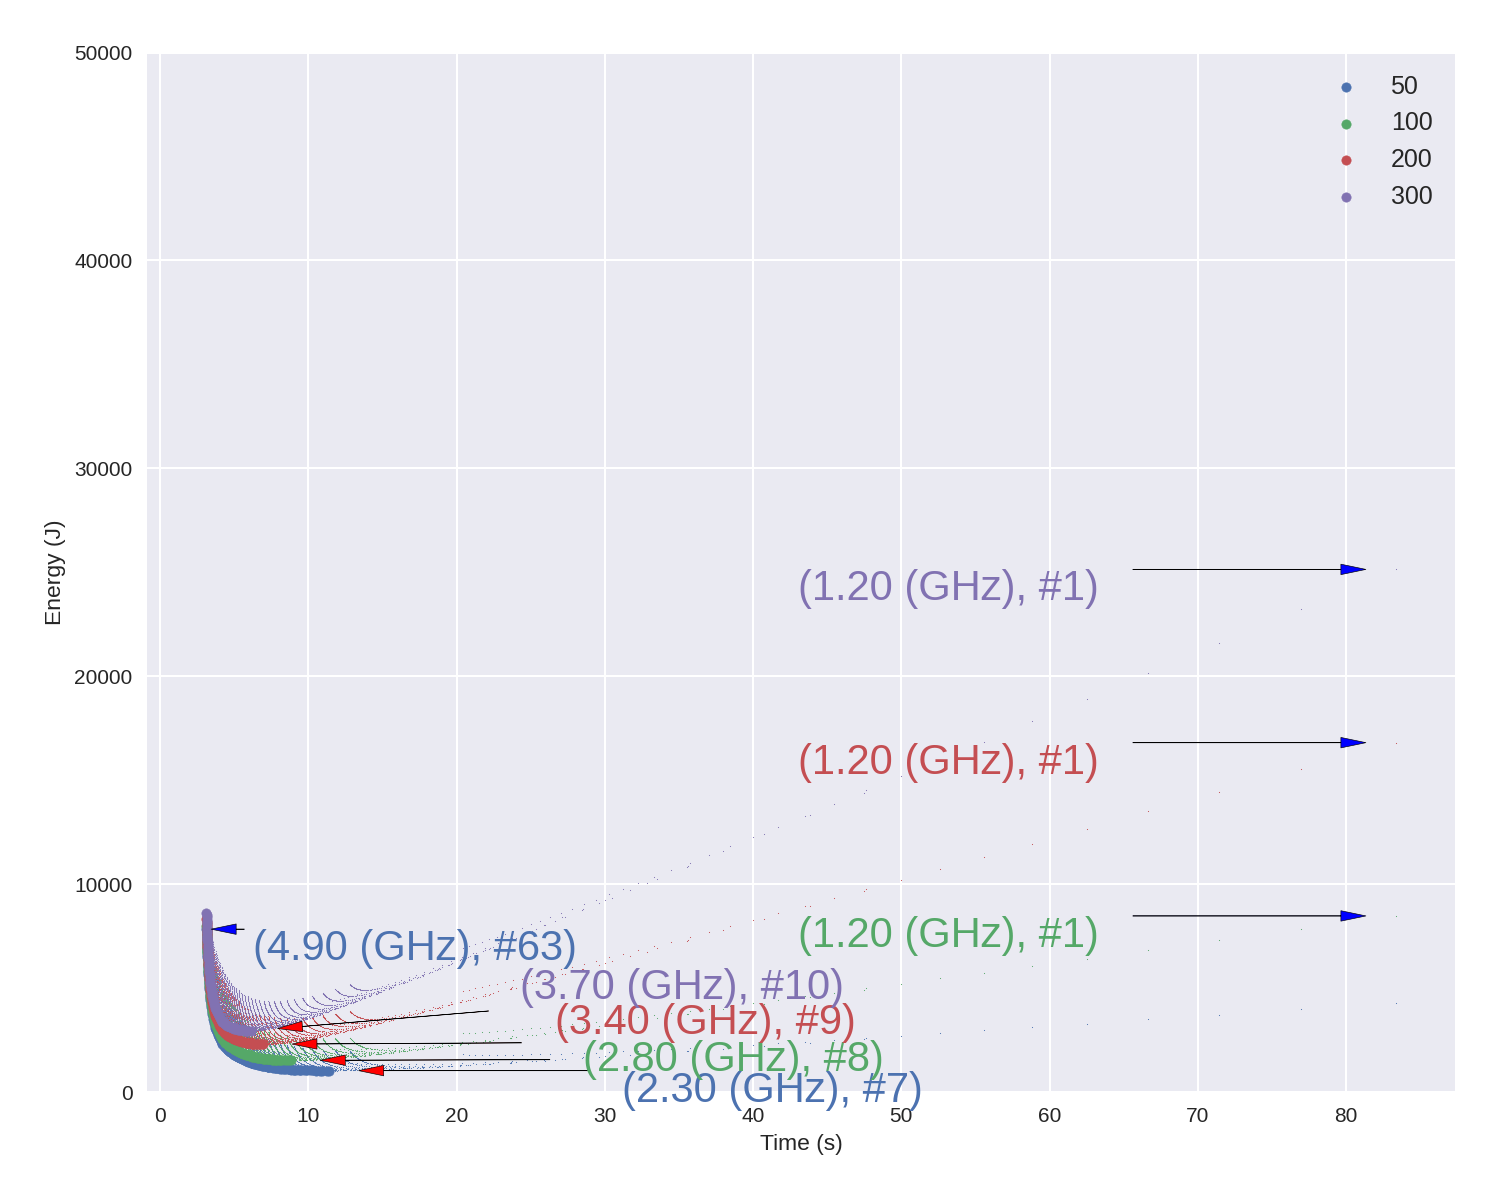
\includegraphics[width=\columnwidth]{models/figures/analisys/pareto_static_high.png}
	\caption{Pareto static energy}
	\label{fig:pareto_static_h}
\end{figure}


\begin{figure}
	\centering
	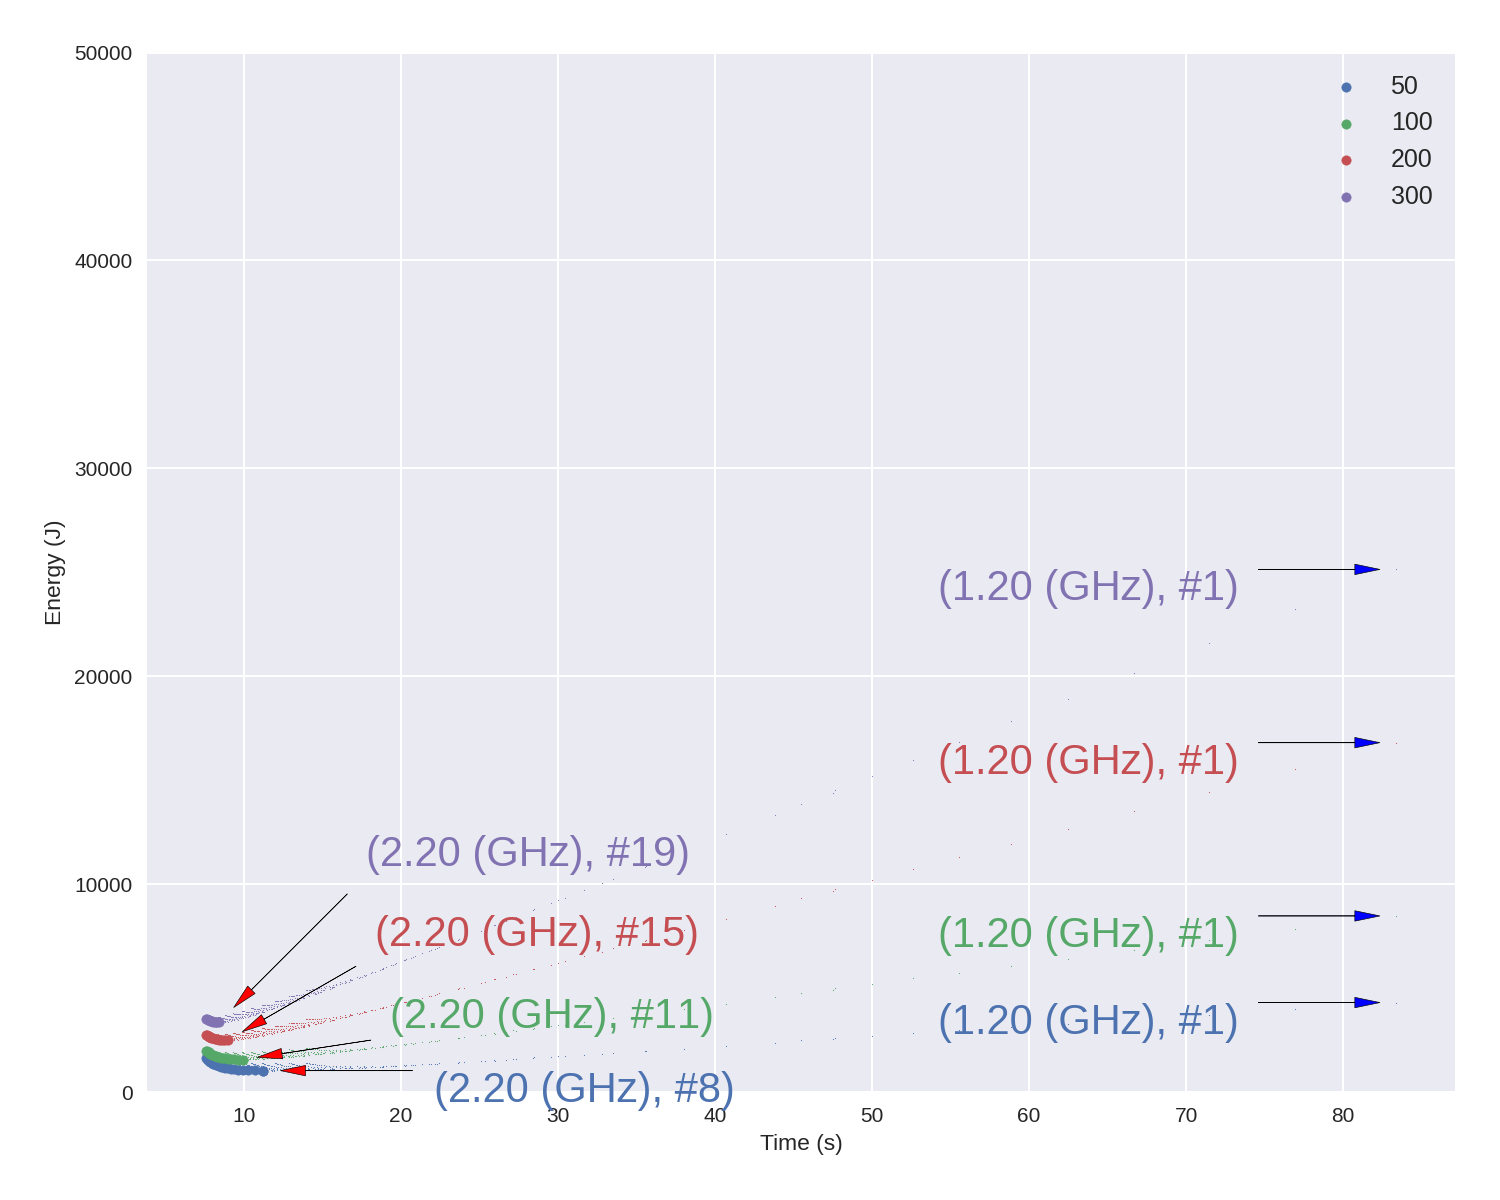
\includegraphics[width=\columnwidth]{models/figures/analisys/pareto_static_low.png}
	\caption{Pareto static energy}
	\label{fig:pareto_static_l}
\end{figure}


\begin{figure}
	\centering
	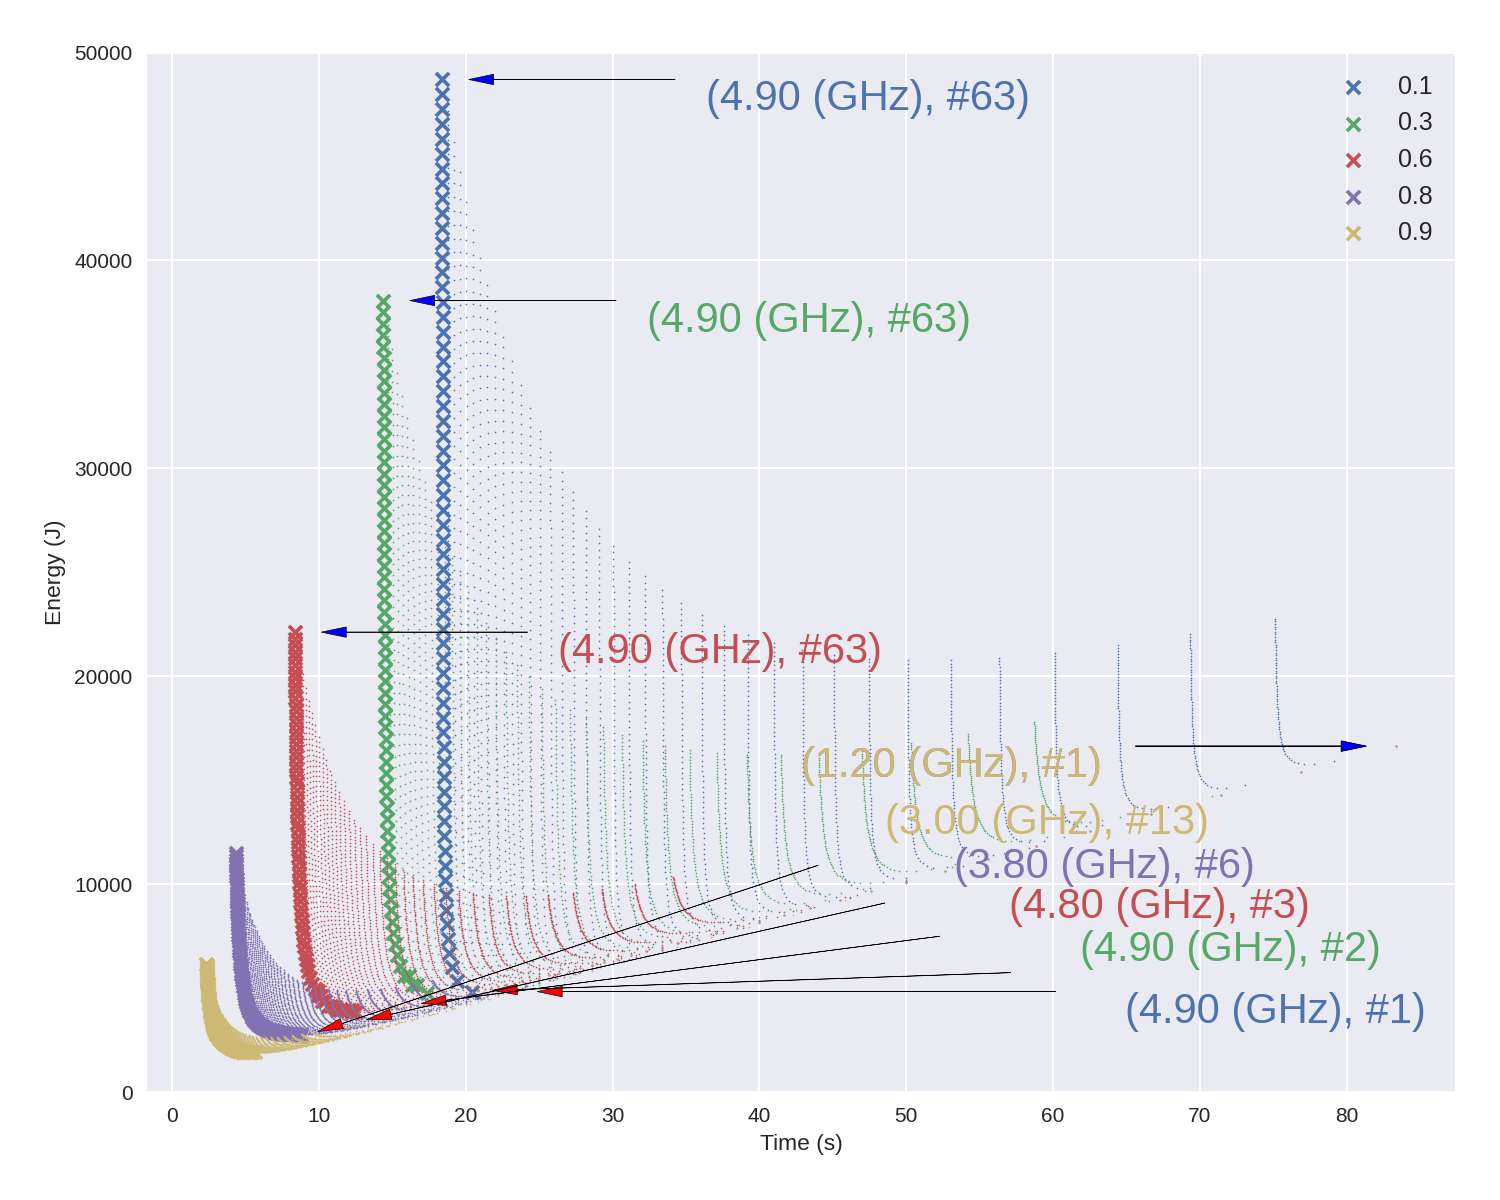
\includegraphics[width=\columnwidth]{models/figures/analisys/pareto_w_high.png}
	\caption{Pareto w energy}
	\label{fig:pareto_w_h}
\end{figure}

\begin{figure}
	\centering
	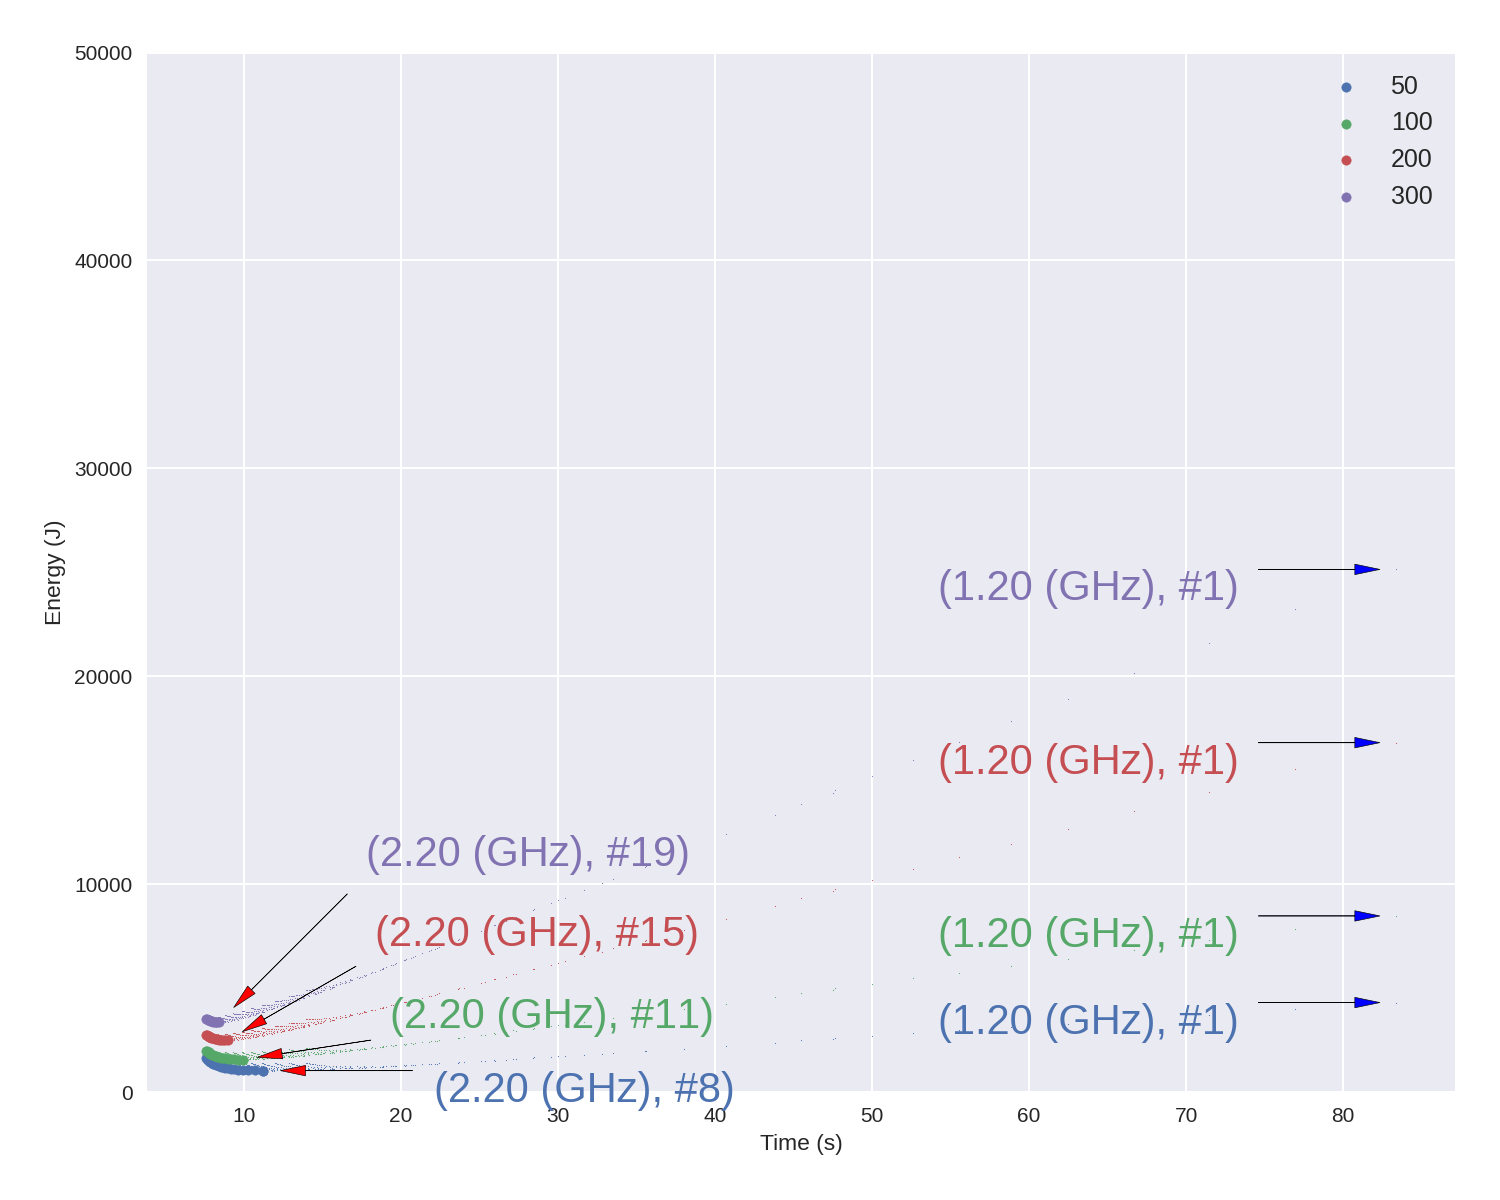
\includegraphics[width=\columnwidth]{models/figures/analisys/pareto_static_low.png}
	\caption{Pareto w energy}
	\label{fig:pareto_w_l}
\end{figure}

\subsection{Optimization under constraints}

\subsection{Gradient and Countorns}

\begin{figure}[H]
	\centering
	\begin{subfigure}[b]{0.45\textwidth}
		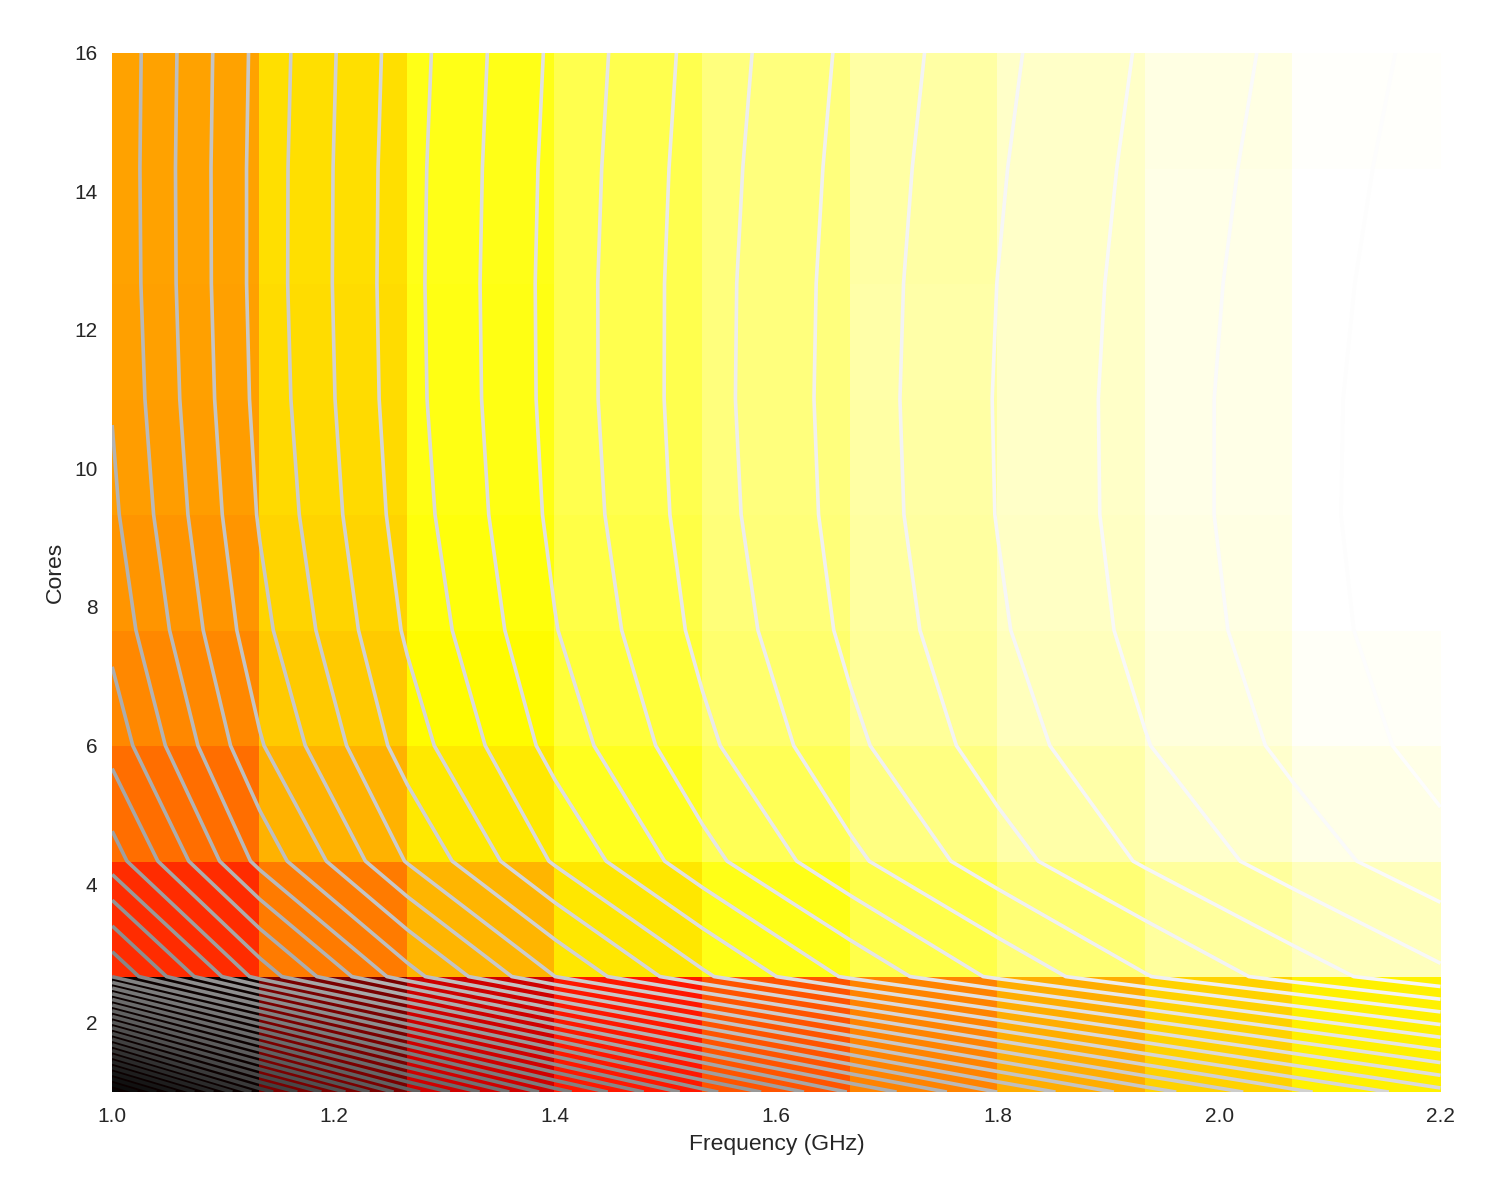
\includegraphics[width=\textwidth]{models/figures/analisys/pdyn0.png}
	\end{subfigure}
	%
	\begin{subfigure}[b]{0.45\textwidth}
		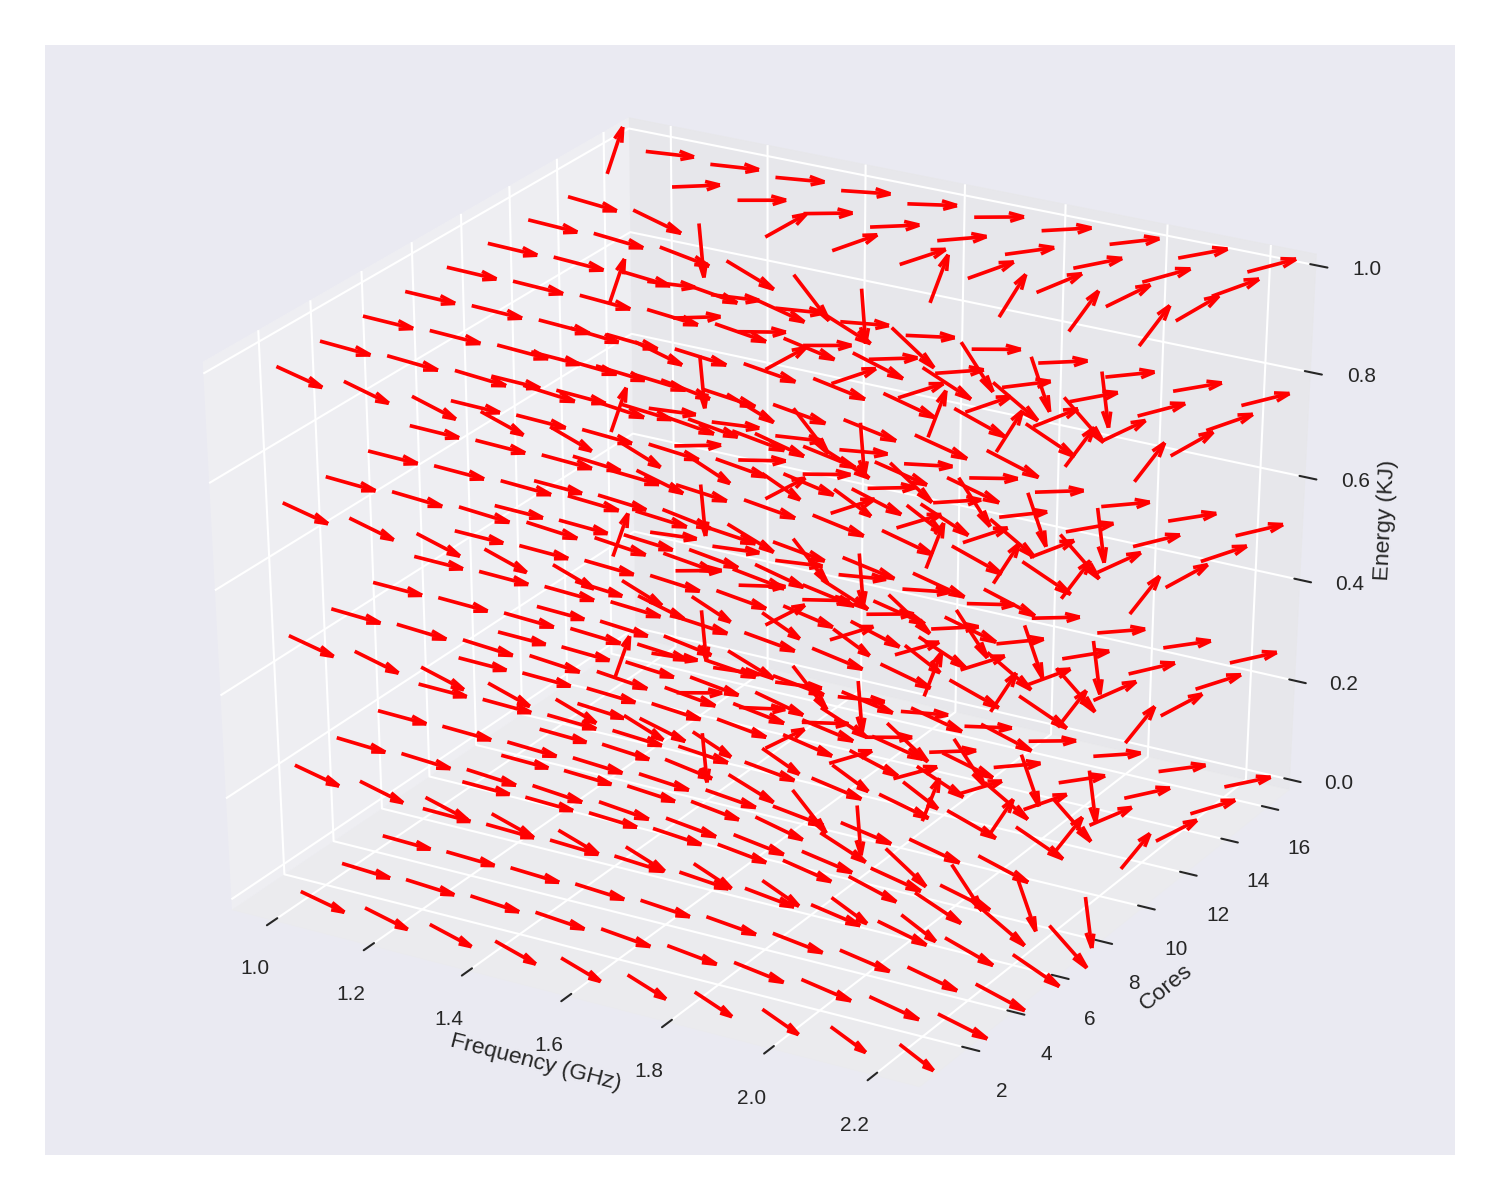
\includegraphics[width=\textwidth]{models/figures/analisys/pdyn0_3d.png}
	\end{subfigure}
\end{figure}

\begin{figure}[H]
	\centering
	\begin{subfigure}[b]{0.45\textwidth}
		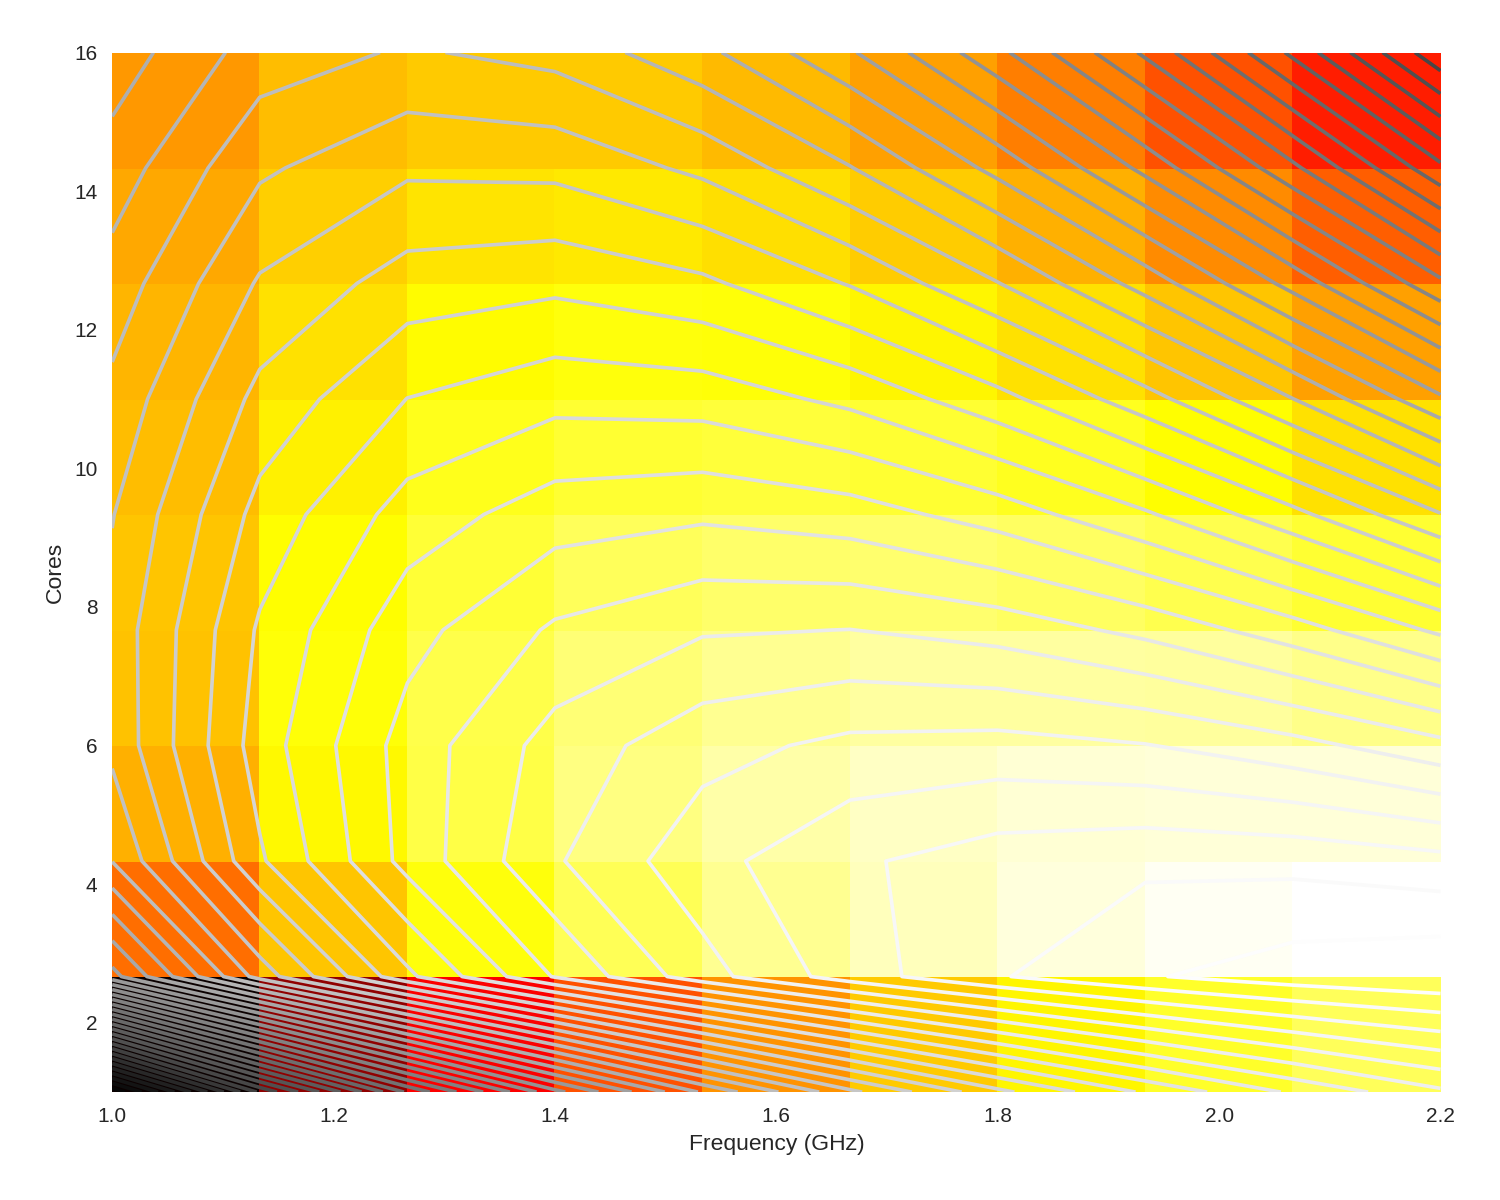
\includegraphics[width=\textwidth]{models/figures/analisys/pdyn3.png}
	\end{subfigure}
	%
	\begin{subfigure}[b]{0.45\textwidth}
		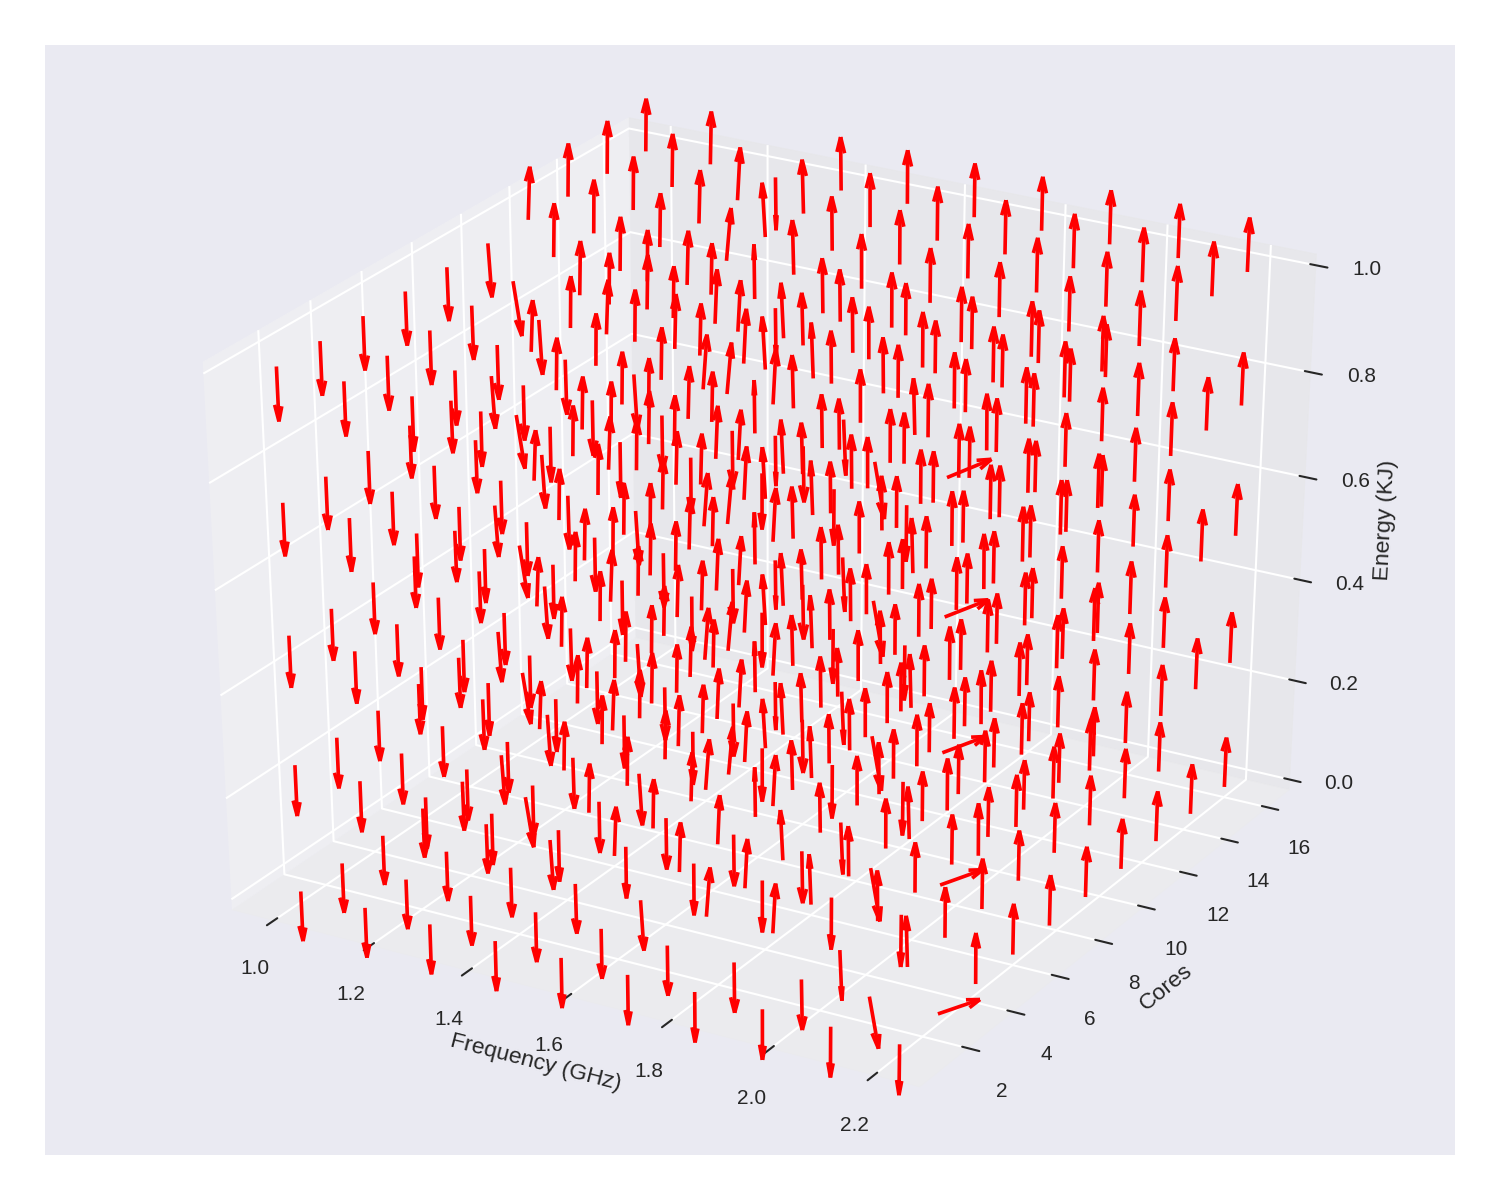
\includegraphics[width=\textwidth]{models/figures/analisys/pdyn3_3d.png}
	\end{subfigure}
\end{figure}

\begin{figure}[H]
	\centering
	\begin{subfigure}[b]{0.45\textwidth}
		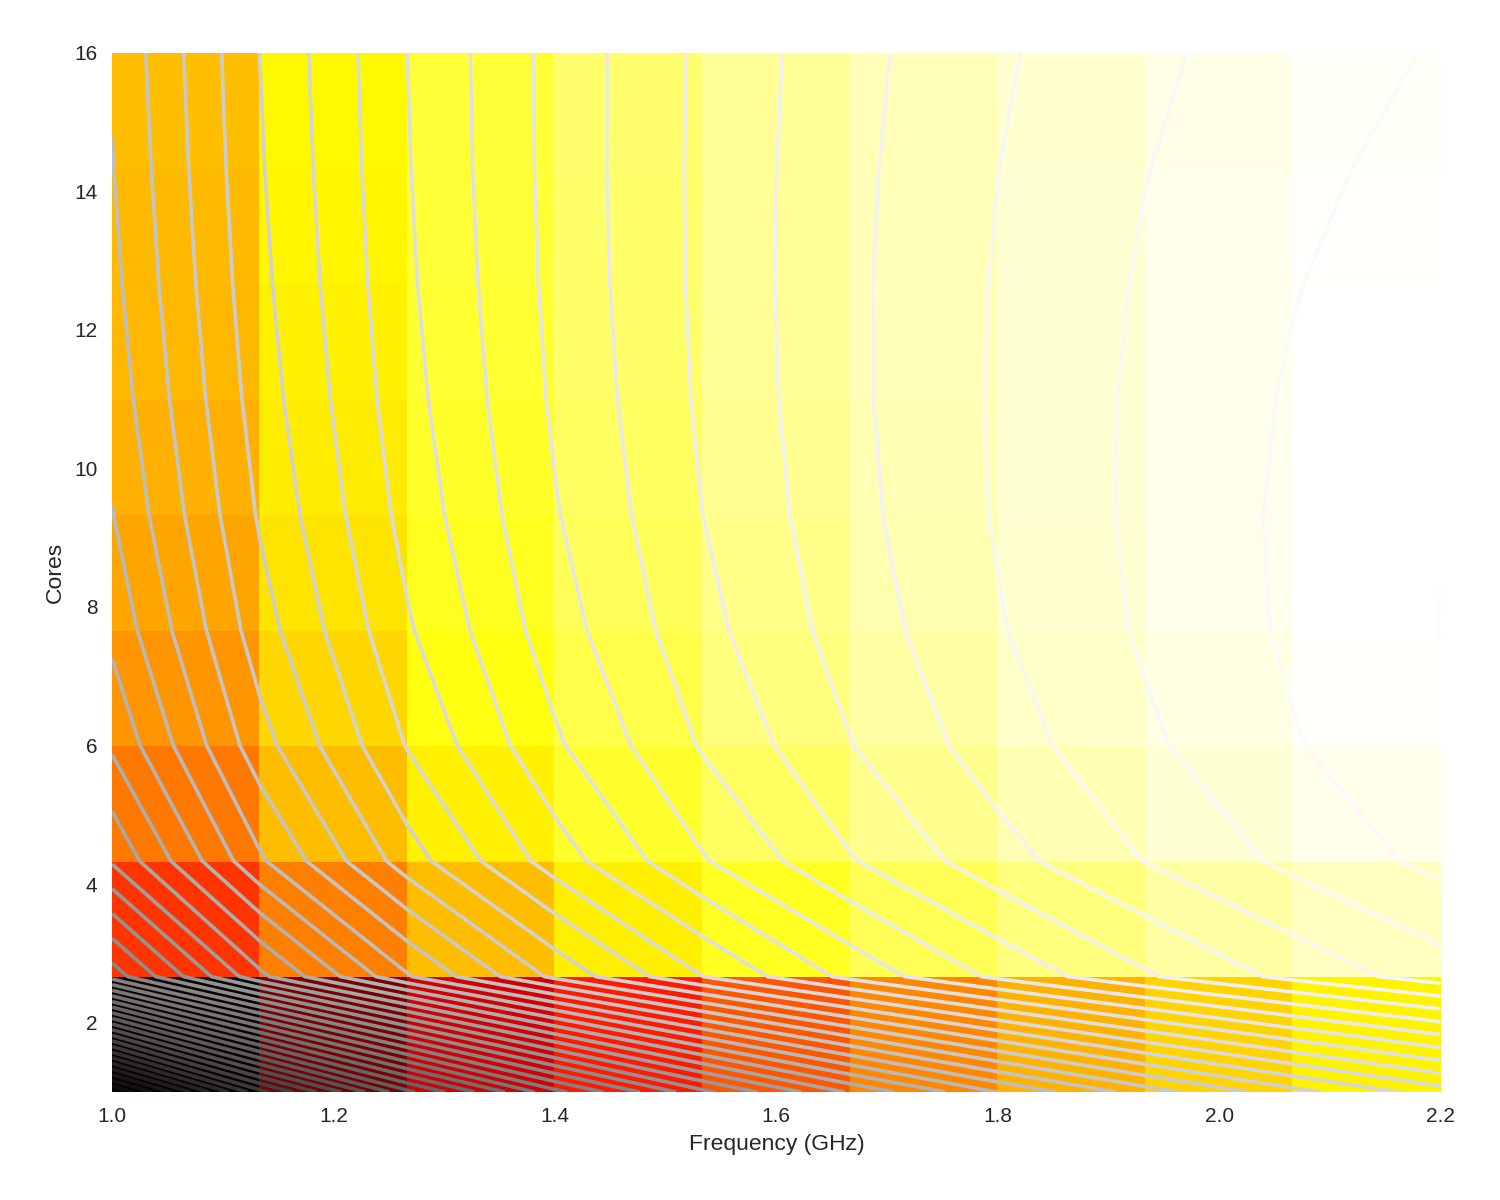
\includegraphics[width=\textwidth]{models/figures/analisys/pleak0.png}
	\end{subfigure}
	%
	\begin{subfigure}[b]{0.45\textwidth}
		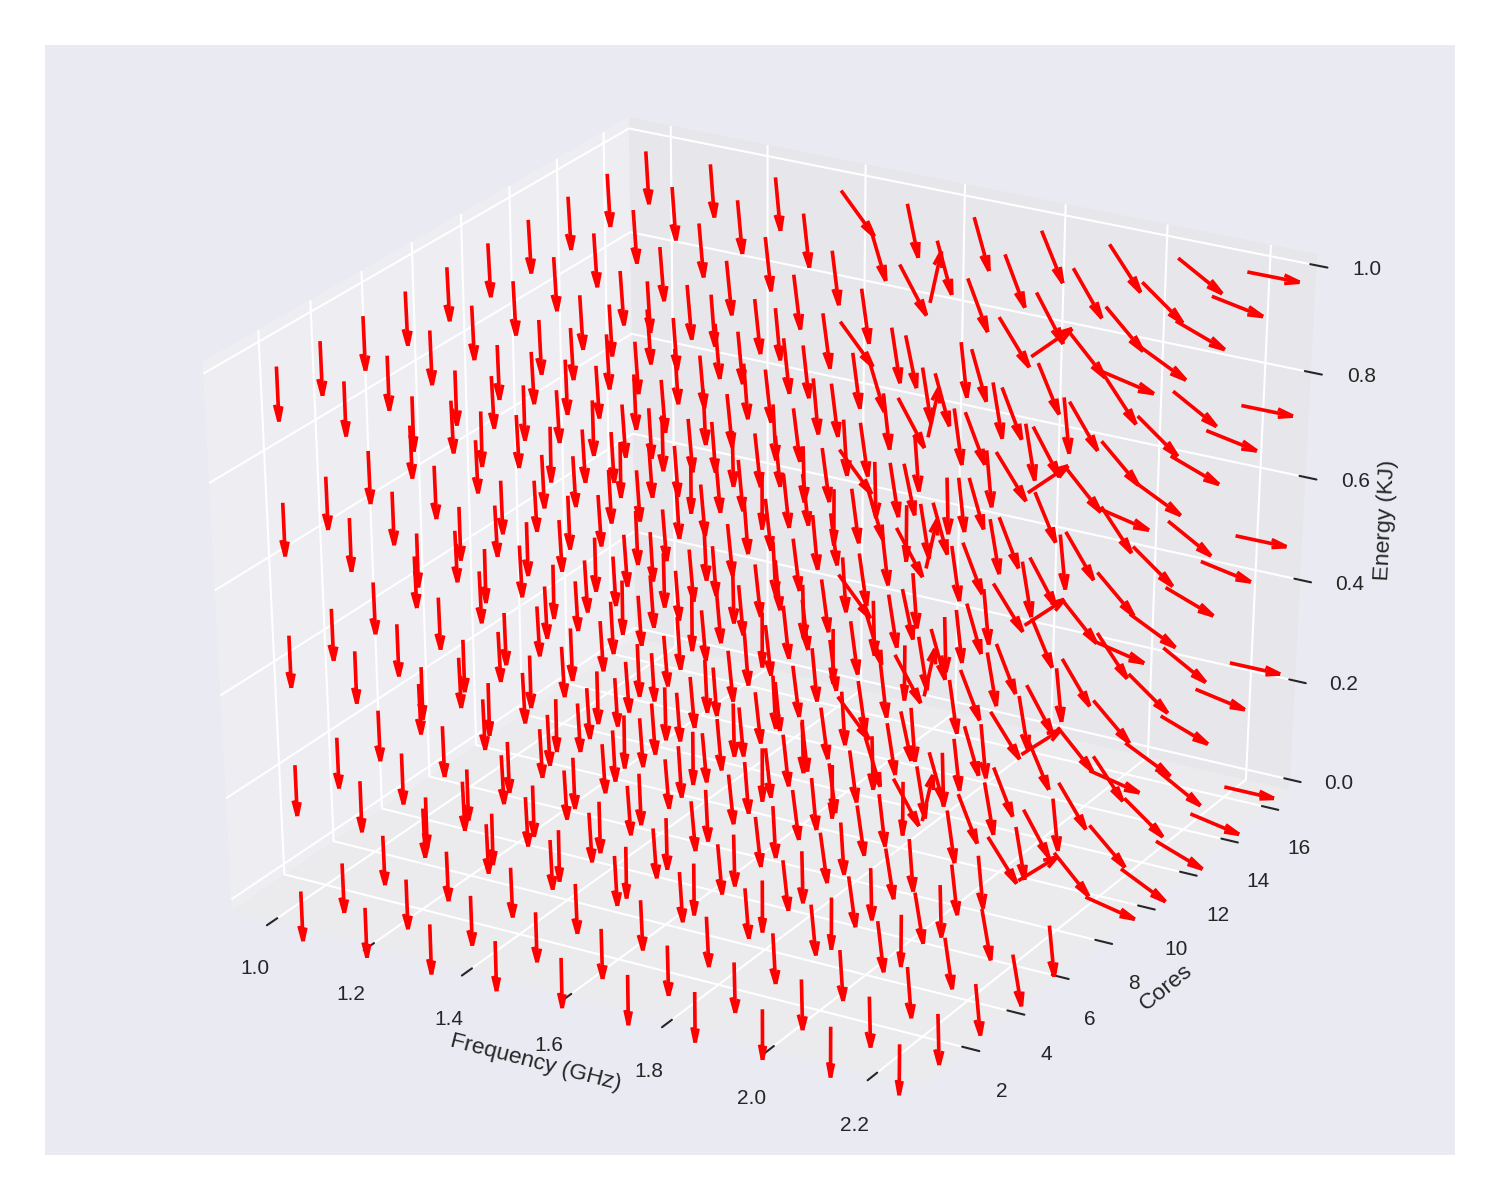
\includegraphics[width=\textwidth]{models/figures/analisys/pleak0_3d.png}
	\end{subfigure}
\end{figure}

\begin{figure}[H]
	\centering
	\begin{subfigure}[b]{0.45\textwidth}
		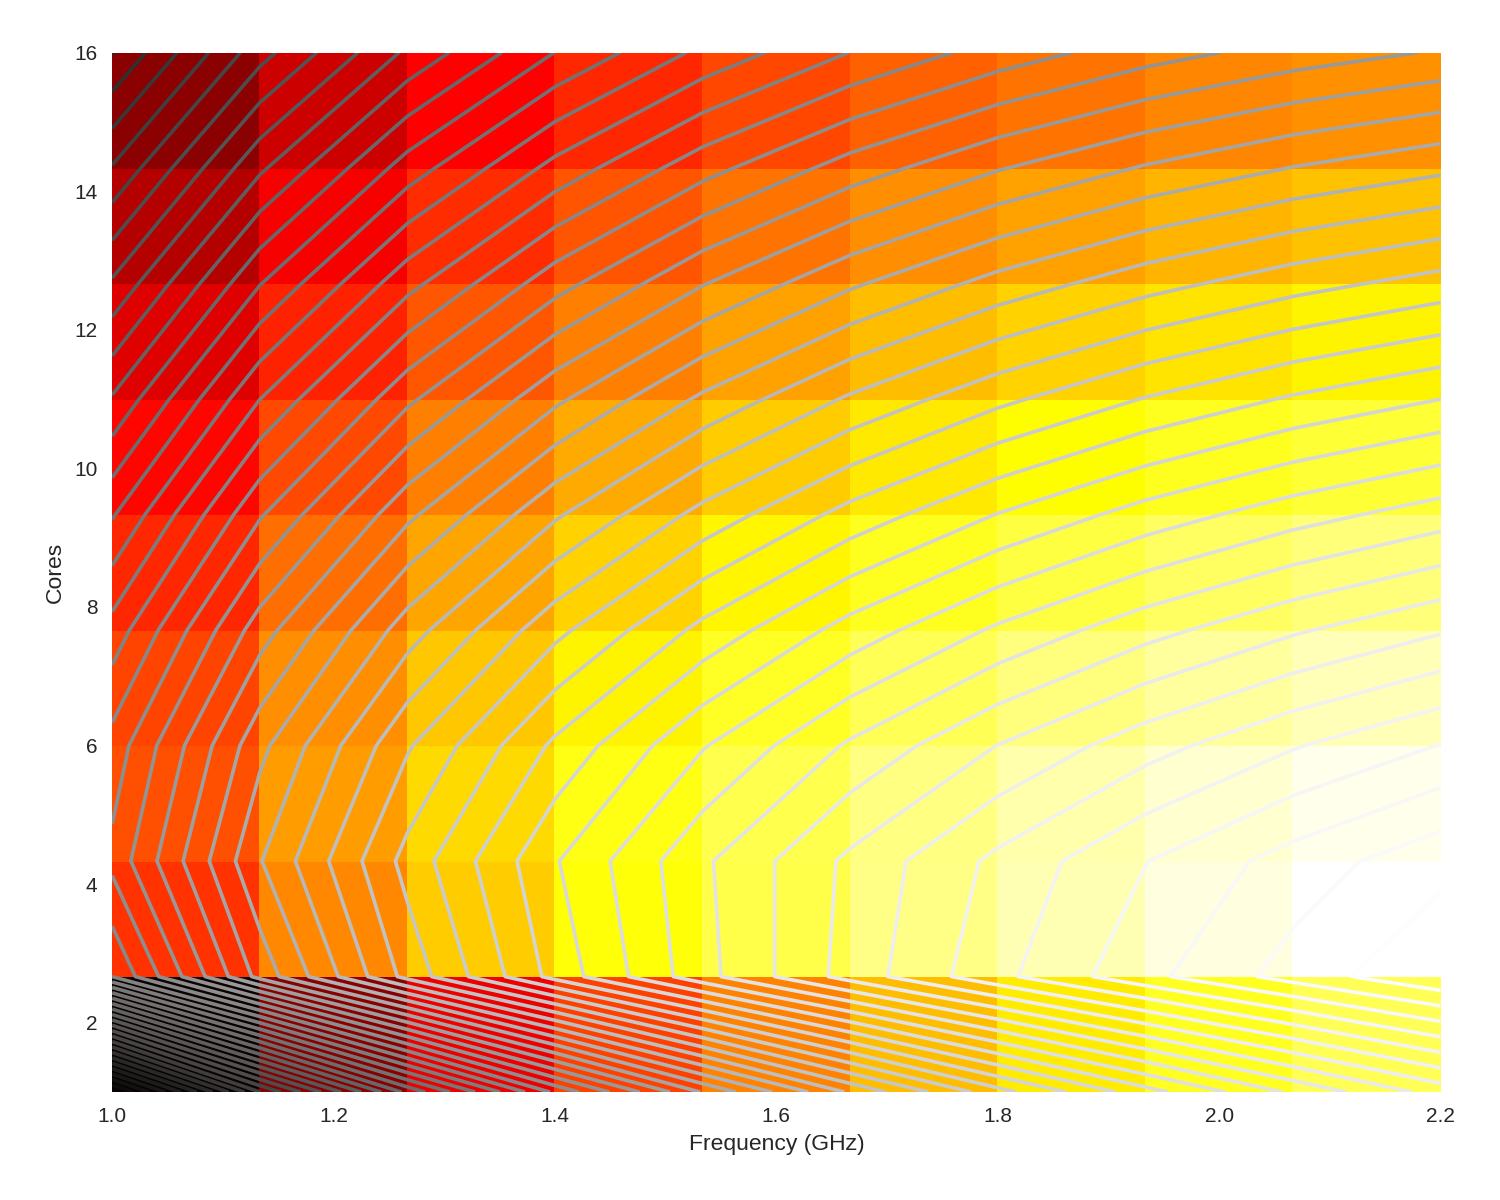
\includegraphics[width=\textwidth]{models/figures/analisys/pleak10.png}
	\end{subfigure}
	%
	\begin{subfigure}[b]{0.45\textwidth}
		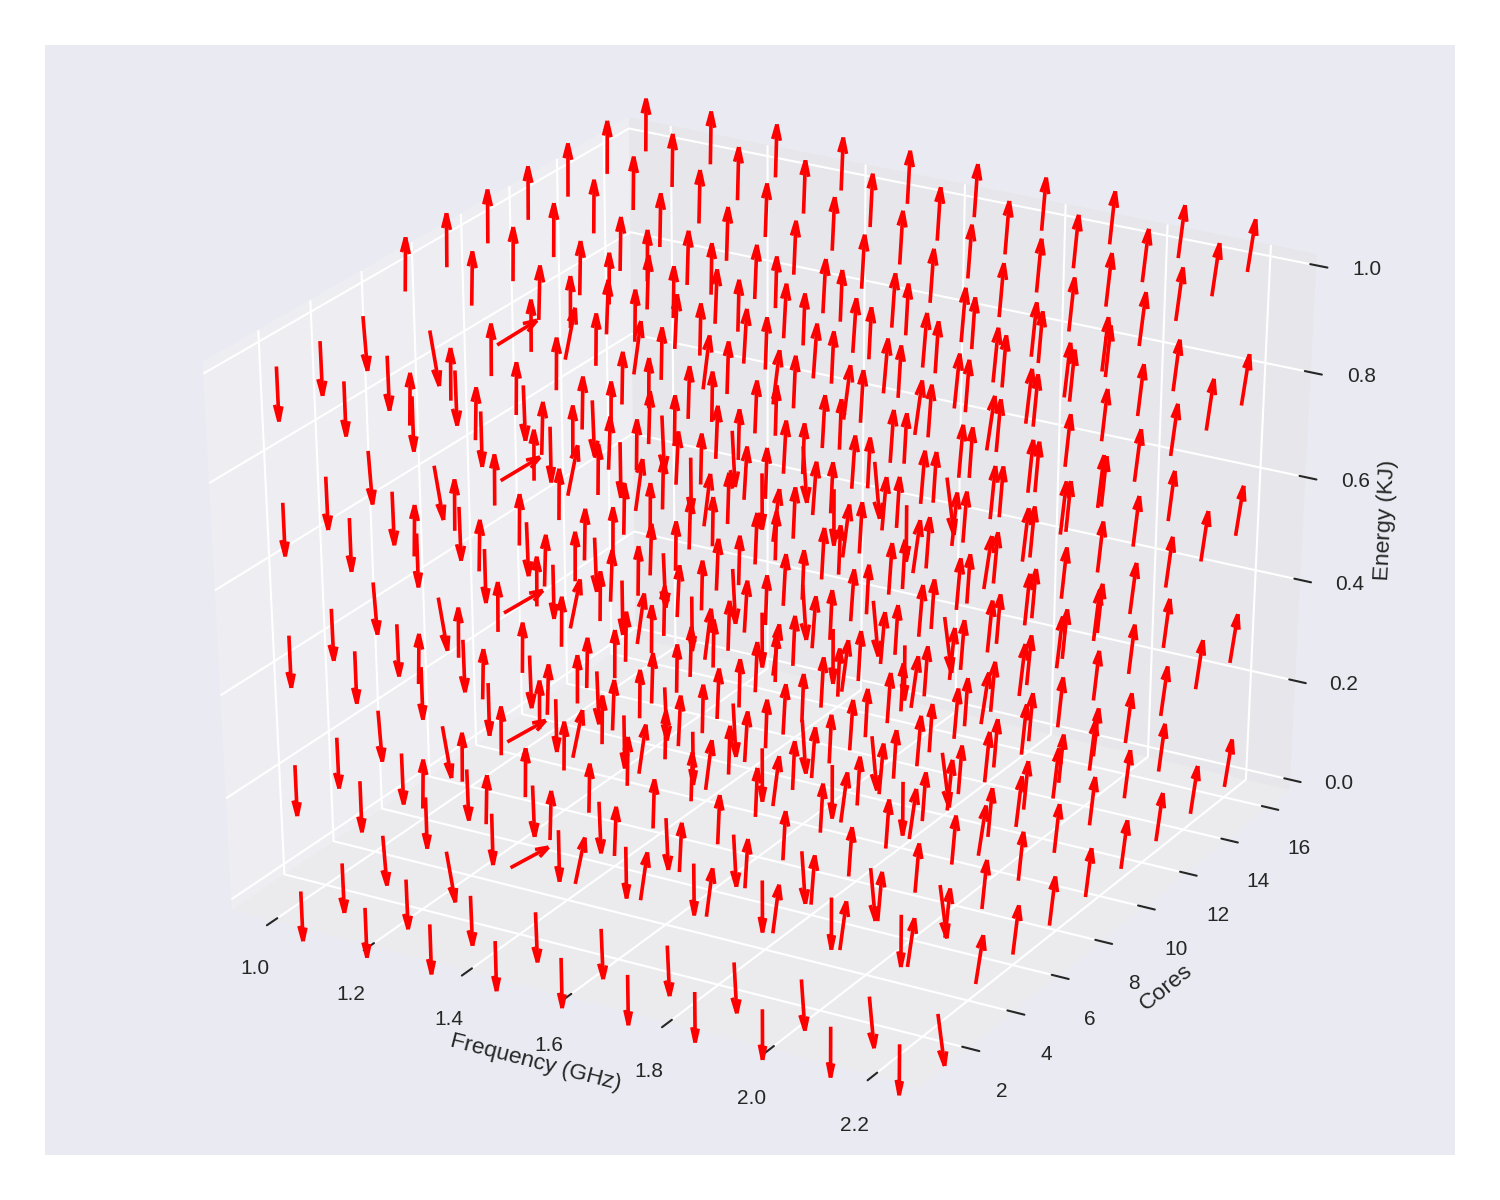
\includegraphics[width=\textwidth]{models/figures/analisys/pleak10_3d.png}
	\end{subfigure}
\end{figure}

\begin{figure}[H]
	\centering
	\begin{subfigure}[b]{0.45\textwidth}
		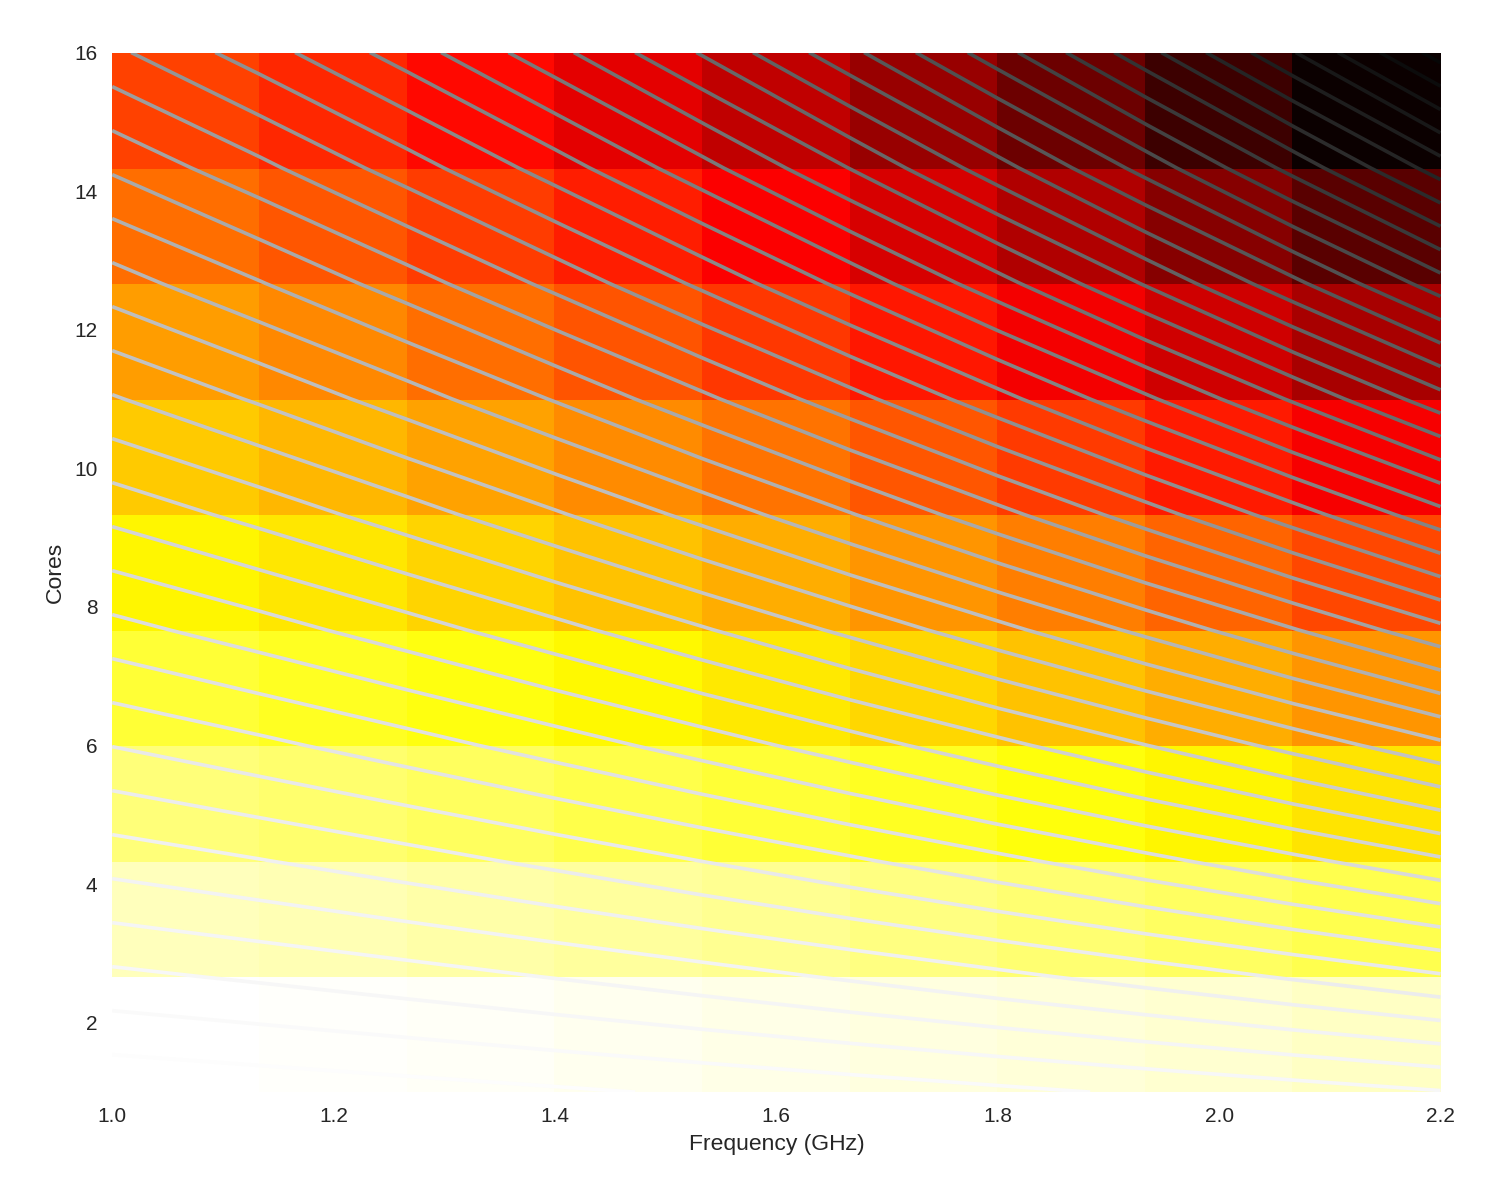
\includegraphics[width=\textwidth]{models/figures/analisys/pstatic0.png}
	\end{subfigure}
	%
	\begin{subfigure}[b]{0.45\textwidth}
		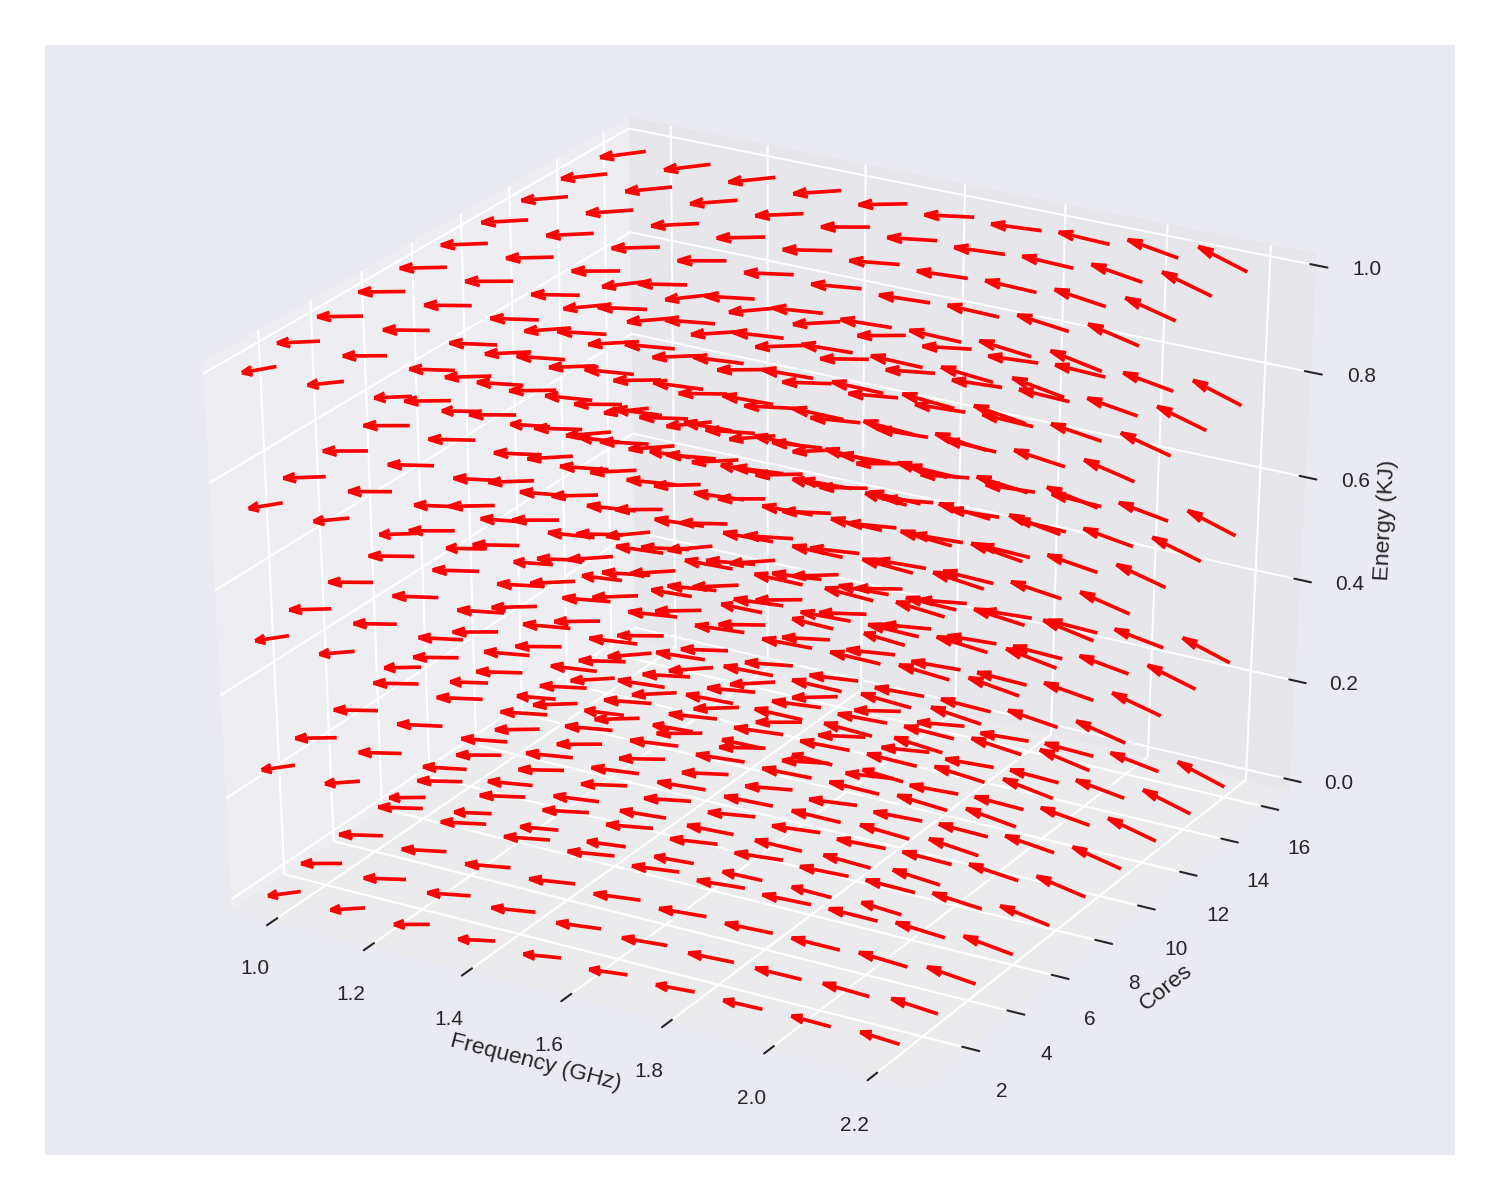
\includegraphics[width=\textwidth]{models/figures/analisys/pstatic0_3d.png}
	\end{subfigure}
\end{figure}

\begin{figure}[H]
	\centering
	\begin{subfigure}[b]{0.45\textwidth}
		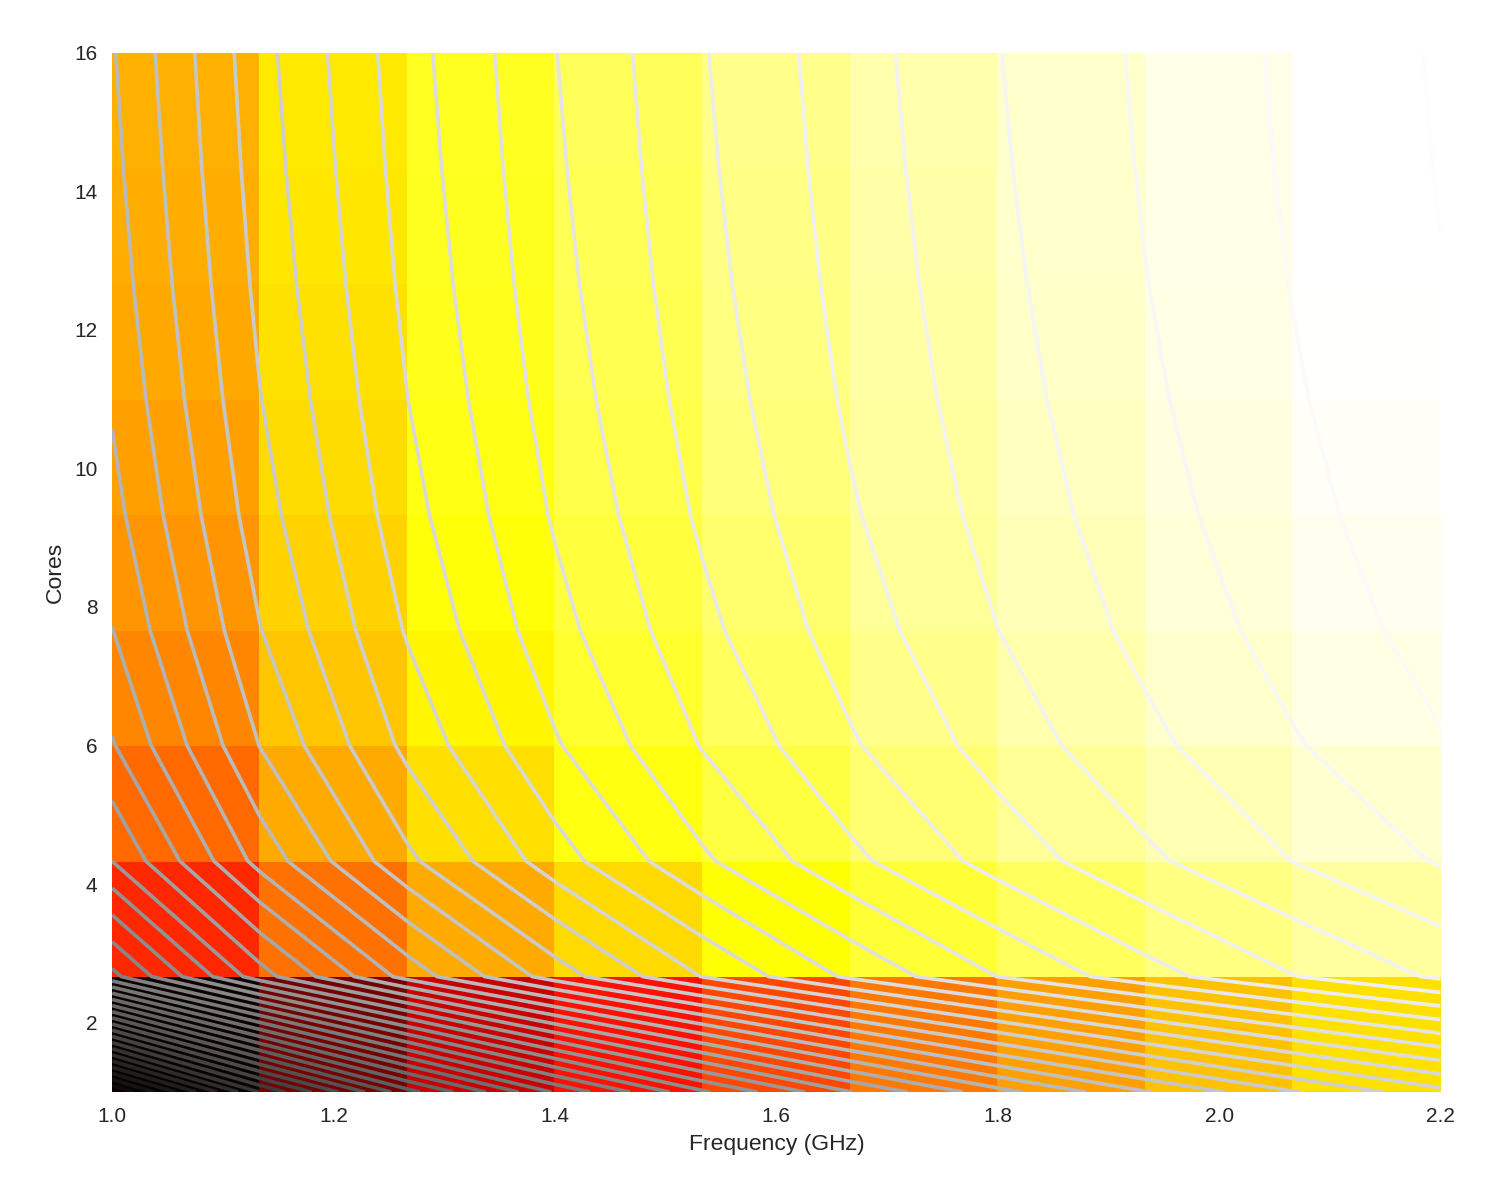
\includegraphics[width=\textwidth]{models/figures/analisys/pstatic3000.png}
	\end{subfigure}
	%
	\begin{subfigure}[b]{0.45\textwidth}
		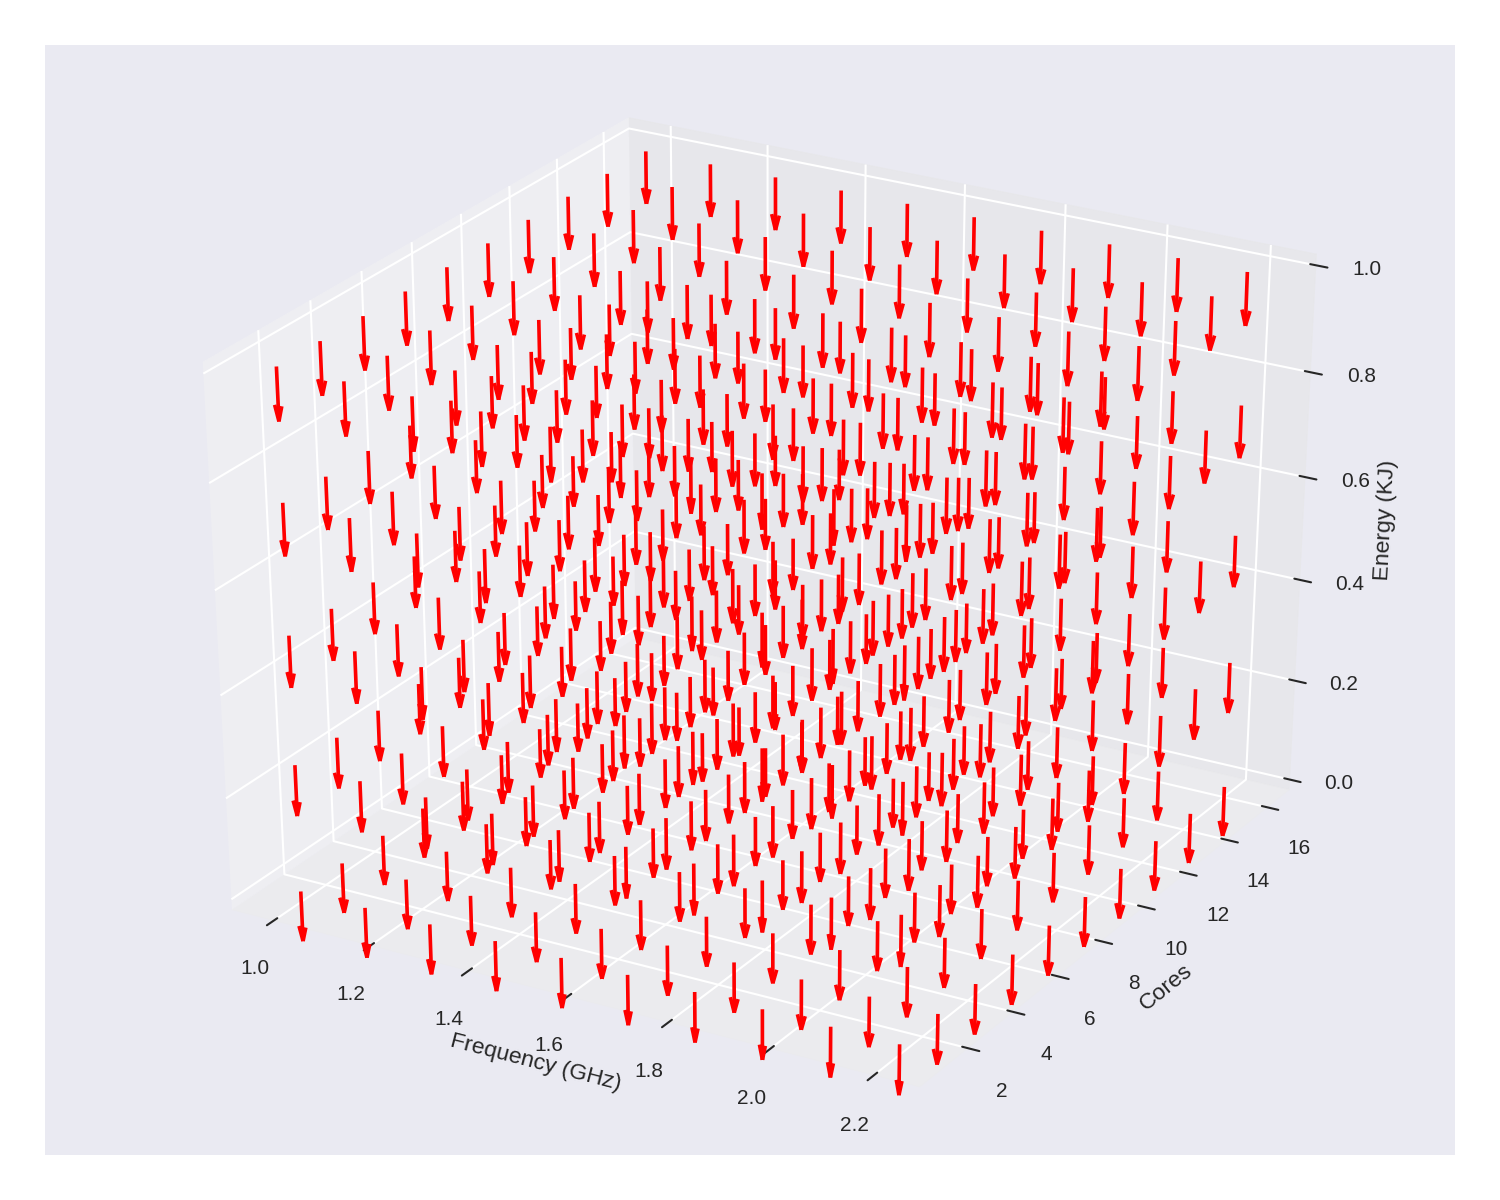
\includegraphics[width=\textwidth]{models/figures/analisys/pstatic3000_3d.png}
	\end{subfigure}
\end{figure}

\begin{figure}[H]
	\centering
	\begin{subfigure}[b]{0.45\textwidth}
		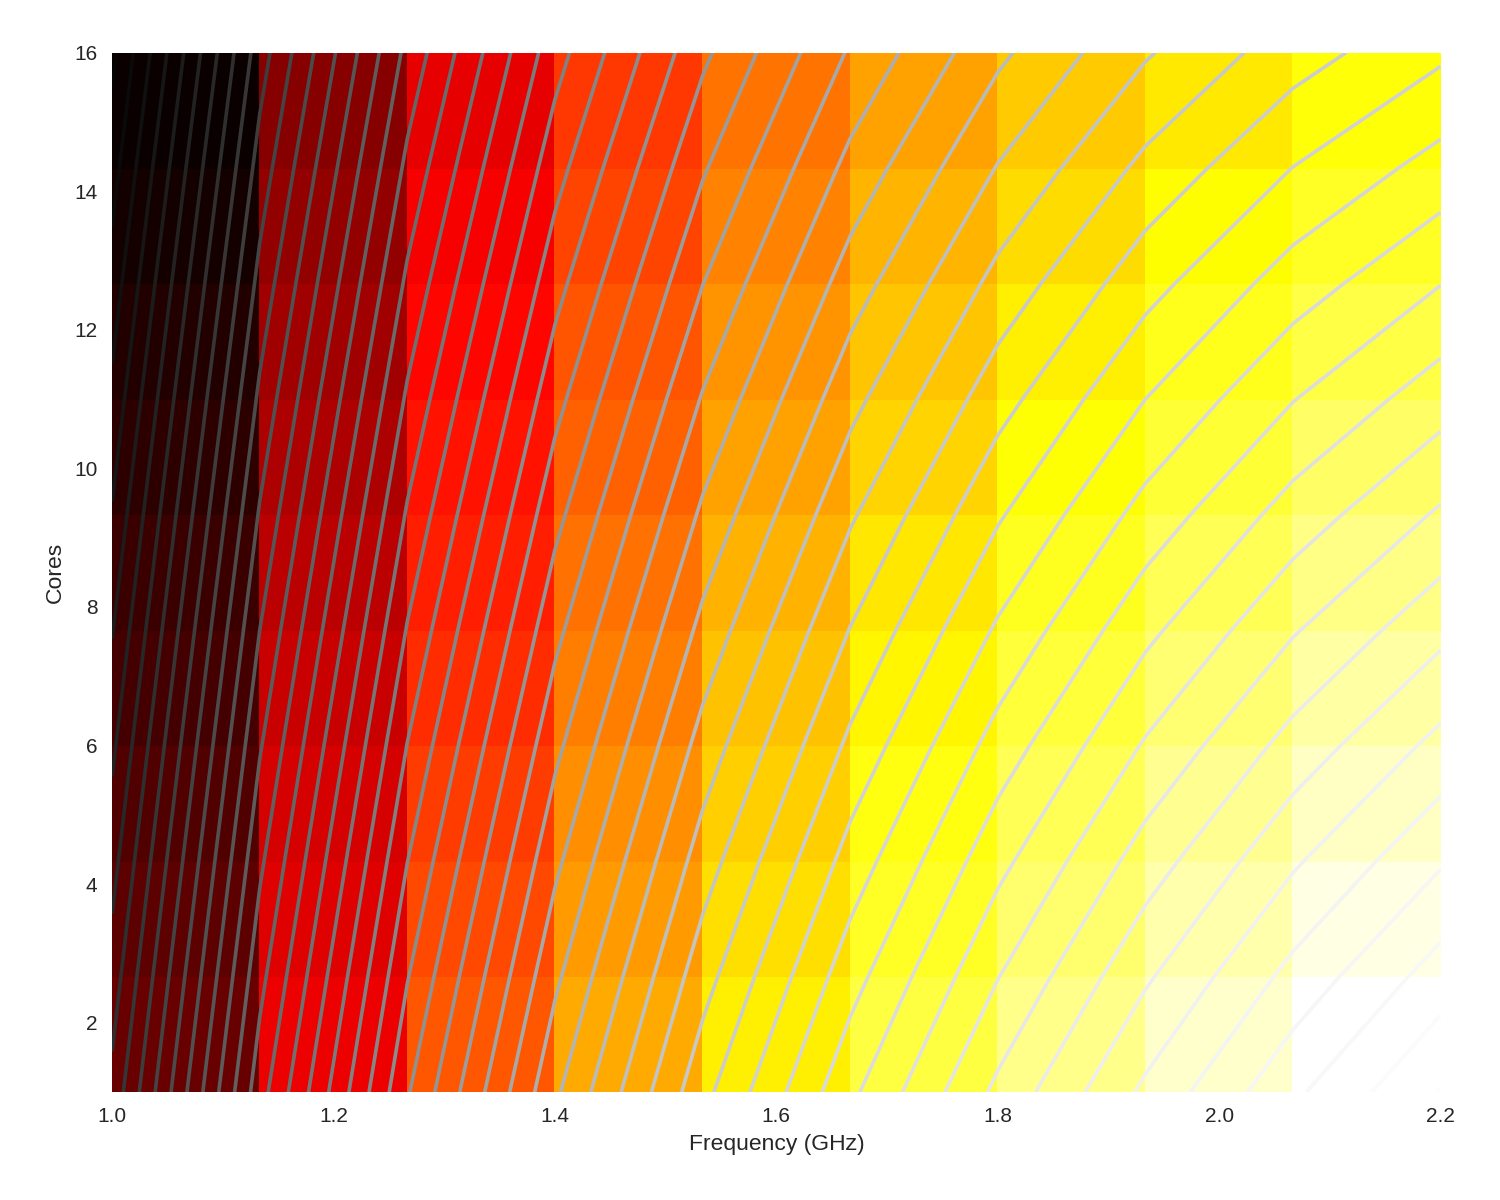
\includegraphics[width=\textwidth]{models/figures/analisys/w0.png}
	\end{subfigure}
	%
	\begin{subfigure}[b]{0.45\textwidth}
		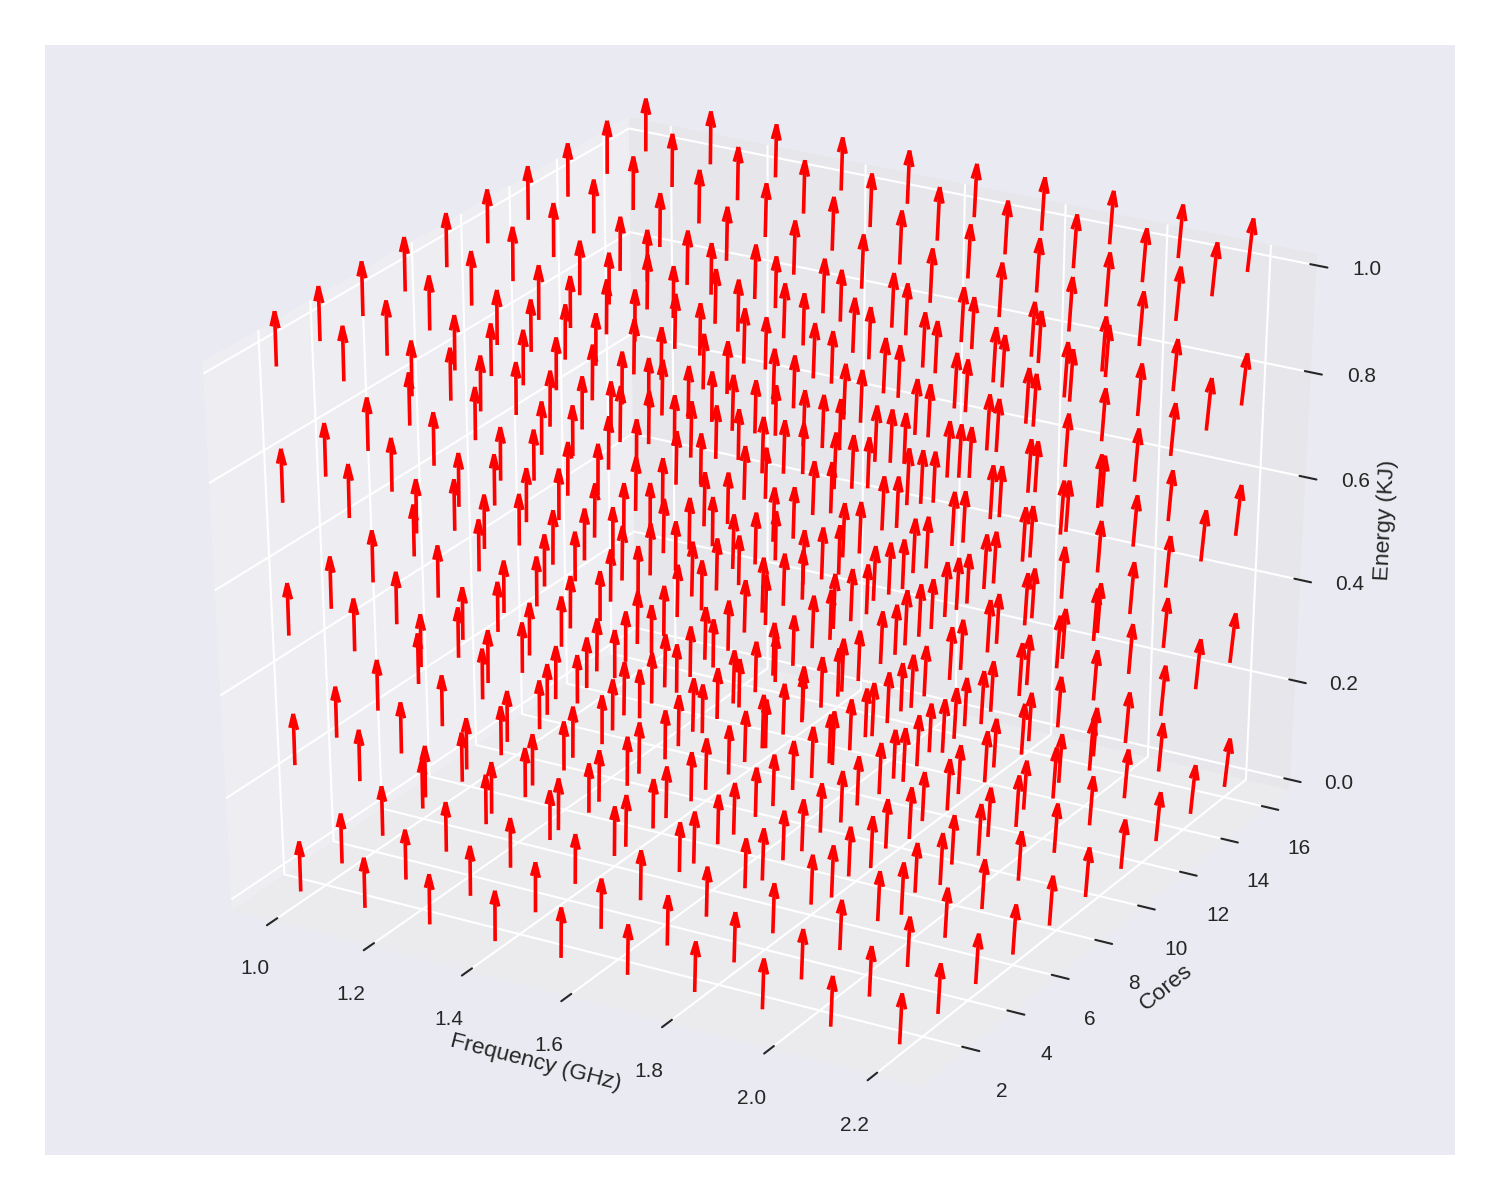
\includegraphics[width=\textwidth]{models/figures/analisys/w0_3d.png}
	\end{subfigure}
\end{figure}

\begin{figure}[H]
	\centering
	\begin{subfigure}[b]{0.45\textwidth}
		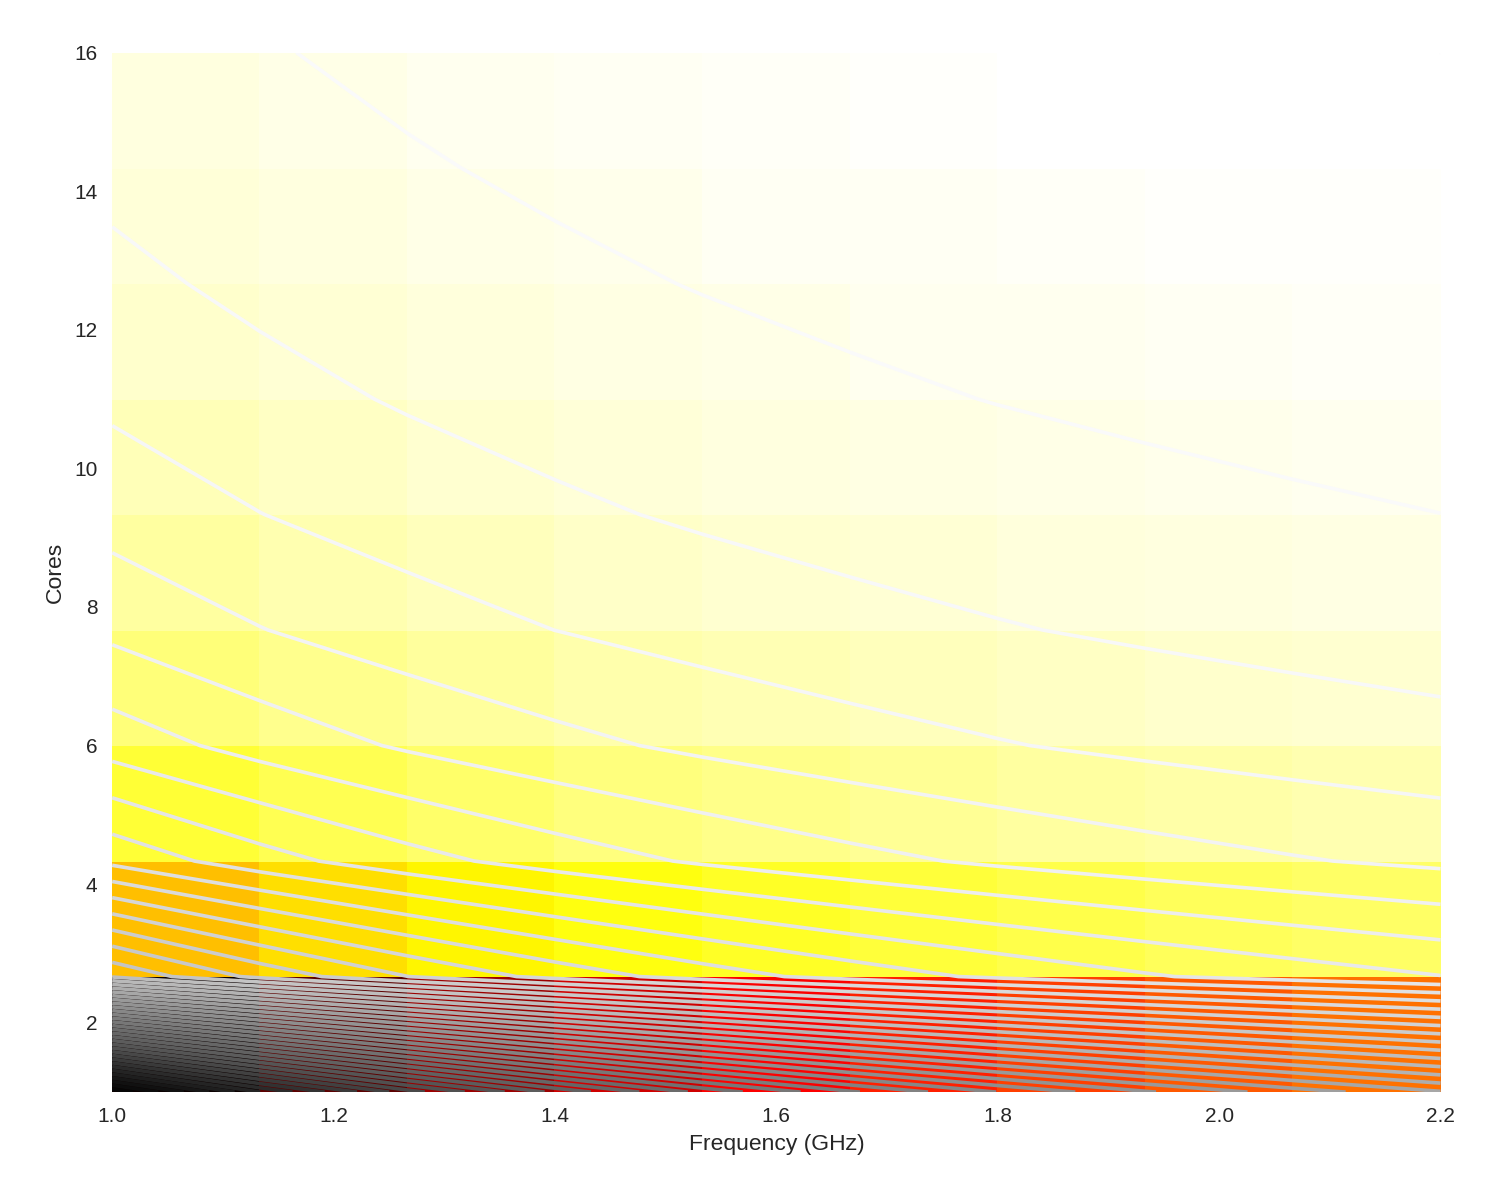
\includegraphics[width=\textwidth]{models/figures/analisys/w1.png}
	\end{subfigure}
	%
	\begin{subfigure}[b]{0.45\textwidth}
		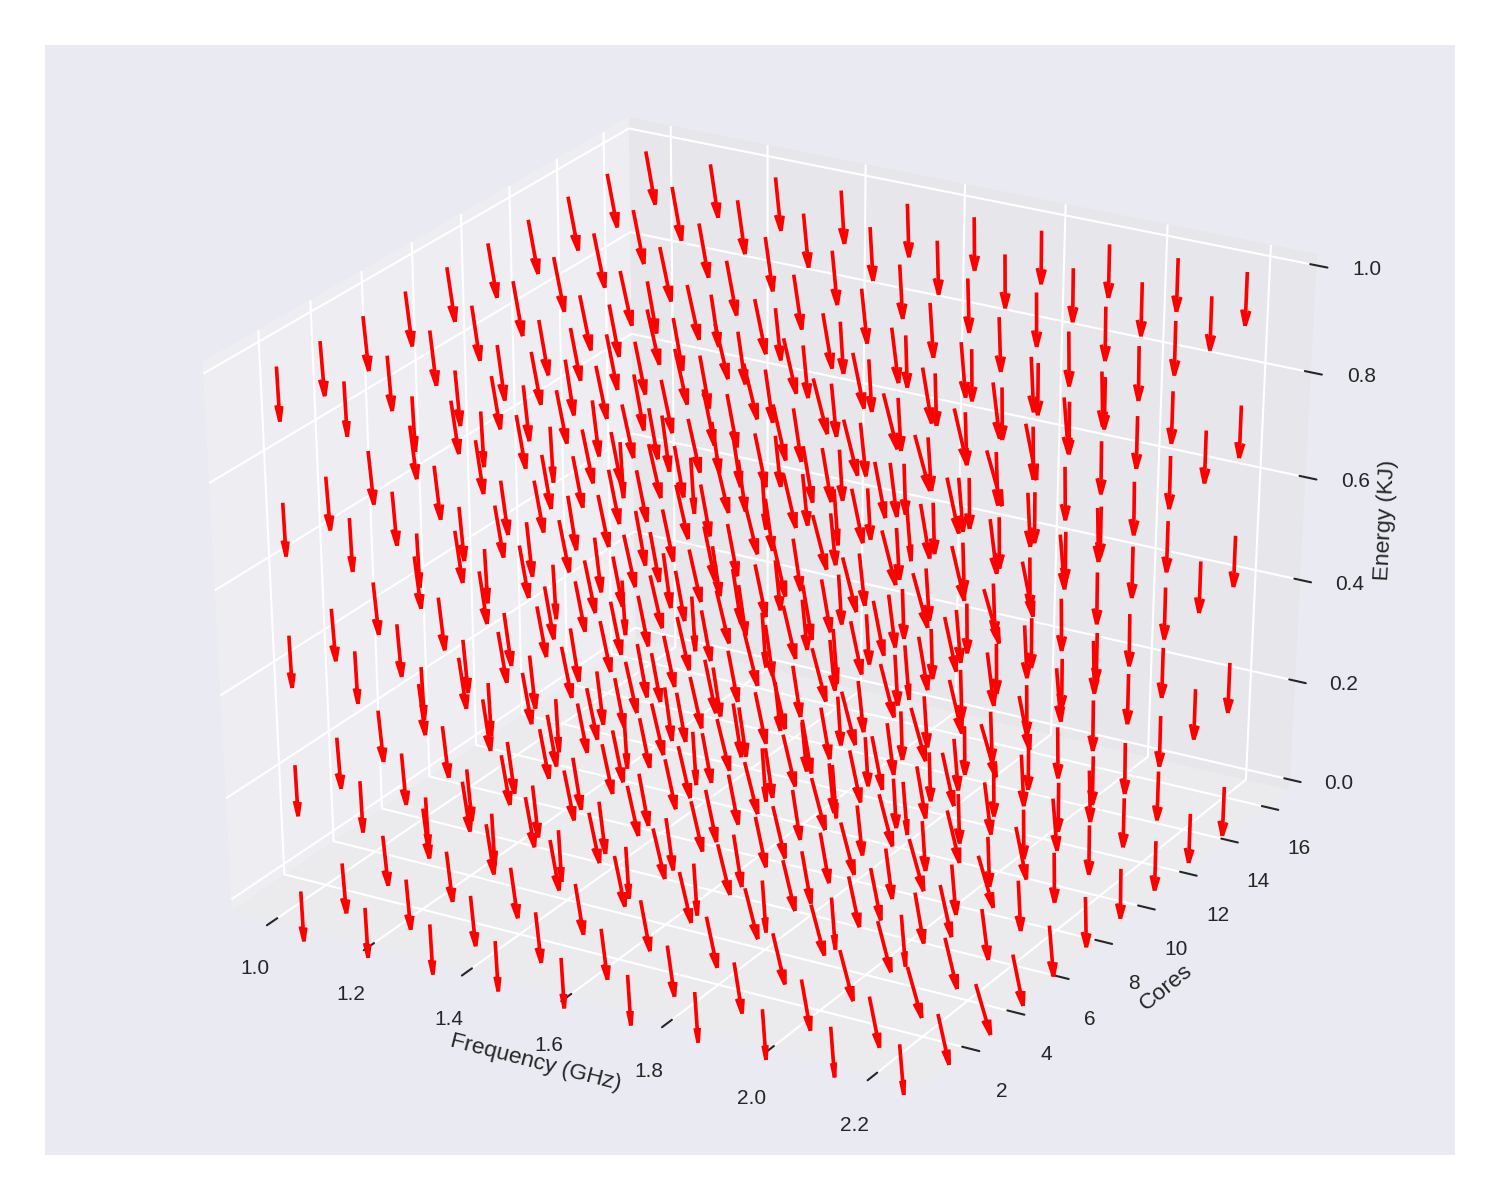
\includegraphics[width=\textwidth]{models/figures/analisys/w1_3d.png}
	\end{subfigure}
\end{figure}
